\documentclass[11pt,a4paper,twoside,openright]{report}

\usepackage{textcomp,gensymb}
% \usepackage[scriptsize]{caption}
\usepackage{subcaption}
\usepackage[dvips]{graphicx}
\usepackage{tabularx}
\usepackage{afterpage}
\usepackage{amsmath,amssymb}
\usepackage{rotating}
\usepackage{fancyhdr}
\hyphenation{a-gen-tiz-za-zio-ne}
% \expandafter\def\csname ver@subfig.sty\endcsname{}
\usepackage{svg}
\usepackage{tikz}
\usetikzlibrary{matrix,chains,positioning,decorations.pathreplacing,arrows}

% \setlength{\paperwidth}{16cm}
% \setlength{\paperheight}{24cm}
\setlength{\oddsidemargin} {2. cm}
\setlength{\evensidemargin} {2. cm}
\addtolength{\oddsidemargin} {-0.4 cm}
\addtolength{\evensidemargin} {-0.4 cm}
\linespread{1.1}

\usepackage[english]{babel}
\usepackage[latin1]{inputenc}
\renewcommand{\captionfont}{\normalfont \sffamily \itshape \small}

\usepackage{listings}
\usepackage{color}

\usepackage{hyperref}
\AtBeginDocument{\def\chapterautorefname{Chapter}}%
\hypersetup{
  colorlinks   = true,    % Colours links instead of ugly boxes
  urlcolor     = black,    % Colour for external hyperlinks
  linkcolor    = black,    % Colour of internal links
  citecolor    = black      % Colour of citations
}


\pagestyle{empty}

\begin{document}
\thispagestyle{empty}
%\begin{titlepage}
\vspace*{-1.5cm} \bfseries{
\begin{center}
  \large
  POLITECNICO DI MILANO\\
  \normalsize
  Corso di Laurea magistrale in Ingegneria Informatica\\
  Dipartimento di Elettronica e Informazione\\
  \begin{figure}[htbp]
    \begin{center}
      
\includegraphics[width=3.5cm]{./pictures/logopm}
%	
\psfig{file=./pictures/logopm.jpg,width=3.5cm}
    \end{center}
  \end{figure}
  \vspace*{0.3cm} \LARGE



  \textbf{A DEEP LEARNING APPROACH TO SUNSPOT DETECTION}\\



  \vspace*{.75truecm} \large
  AI \& R Lab \\
  Laboratorio di Intelligenza Artificiale \\
  e Robotica del Politecnico di Milano
\end{center}
\vspace*{3.0cm} \large
\begin{flushleft}


  Relatore: Ing. Matteo Matteucci \\
  Correlatore: Prof. Tizio, Caio e Sempronio

\end{flushleft}
\vspace*{1.0cm}
\begin{flushright}


  Tesi di Laurea di:\\ Enrico Fini, matricola 860761\\


\end{flushright}
\vspace*{1.0cm}
\begin{center}



  Anno Accademico 2018-2019
\end{center} \clearpage
}

\thispagestyle{empty} \normalfont \cleardoublepage
\vspace{17cm}

%\large
\begin{flushright}
\itshape{ A pap\`{a} e mamma}
\end{flushright}

\thispagestyle{empty}  \cleardoublepage
\pagenumbering{Roman}
\newpage
\chapter*{Sommario}

\addcontentsline{toc}{chapter}{Sommario}

\noindent LO SCRIVO ALLA FINE  \\

\newpage
\chapter*{Abstract}

\addcontentsline{toc}{chapter}{Abstract}

\noindent The strong influence of the Sun on the environment of the Earth makes it necessary to monitor and predict its activity. Sunspots, manifestations of strong pertubations in the magnetic field of the Sun, are one of the visible features that can be studied in order to model solar activity cycles. So far, sunspot counting has been mostly done by humans and the scientific comunity seems reluctant to the introduction of algorithms because they would create a discontinuity with traditional observations. The purpose of this thesis, which lays at the intersection of observational solar physics and cutting-edge computer science, is to demonstrate that, using deep learning, it is possible to build a program capable of learning from expert scientists and performing solar image annotation automatically, according to human criteria. Test cases were designed to assess the quality of our solution with respect to average human performance. The results are promising and show that the algorithm can capture the progress of the solar cycle, making it a good tool for the estimation of the activity of the Sun.

\thispagestyle{empty} \vspace*{.75truecm} \cleardoublepage
\chapter*{Ringraziamenti}

\addcontentsline{toc}{chapter}{Ringraziamenti}

Ringrazio i miei genitori per avermi dato tutto quello che potevano. Sono loro che mi hanno permesso di fare le esperienze all'estero che hanno reso questa laurea magistrale molto pi\`{u} divertente.\\
Ringrazio il Prof. Matteucci per avermi rassicurato e incoraggiato nei momenti in cui pensavo di non farcela. Ricorder\`{o} sempre le sue email alle 2 di notte che mi facevano dormire sonni pi\`{u} tranquilli.\\
Ringrazio gli amici che mi sono stati vicini, in particolare i PdN che hanno condiviso con me questo tortuoso percorso di studi, fatto di sacrifici, successi e tanta birra (tranne il Gingio che \`{e} astemio). Un pensiero speciale va anche a Marco e Fabio, compagni di epiche avventure in Spagna.\\
Un ringraziamento enorme va a Maria, che mi ha sopportato nei momenti di maggiore stress ed ha sofferto con me durante la scrittura della tesi.

\thispagestyle{empty} \vspace*{.75truecm} \normalfont \cleardoublepage
\pagestyle{plain}\renewcommand{\chaptermark}[1]{\markboth{\chaptername\ \thechapter.\ #1}{}}
\renewcommand{\sectionmark}[1]{\markright{\thesection.\ #1}}
\fancyhead[LE,RO]{\bfseries\thepage}

\fancyhead[RE]{\bfseries\leftmark}
\fancyhead[LO]{\bfseries\rightmark}
\renewcommand{\headrulewidth}{0.3pt}
\tableofcontents
% \listoffigures
\cleardoublepage
\pagenumbering{arabic}
% \chapter{Introduzione}
\label{Introduzione}
\thispagestyle{empty}

\noindent LO SCRIVO ALLA FINE

% \chapter{Background}
\label{capitolo2}
\thispagestyle{empty}


\noindent The Sun is the closest star to the Earth and it sits at the heart of the Solar System. It is by far the largest object of our surroundings, in fact our planet can fit more than a million times in its volume \cite{Laclare1996} while it holds 99.86\% of the total mass of the Solar System \cite{astro-const} and its magnetic field reaches well past Pluto and Neptune \cite{nasa-sun-earth}. The activity of the Sun has significant environmental influences on the Earth and therefore modeling its behaviour is fundamental. In order to do that it is necessary to understand its structure first, since a great deal of the phenomena that take place in the outer parts of a star are actually caused by some internal mechanism. The Standard Solar Model (SSM) \cite{ssm} is a mathematical formalization of the functioning of the Sun. It can be used to predict the internal observables (physical quantities that can be measured) through the resolution of the classical stellar equations and the knowledge of fundamental physics like nuclear reaction rates, screening, photon interaction, plasma physics \cite{ssmb}. In recent times, thanks to GOLF, MDI, and VIRGO instruments aboard SOHO \cite{soho} spacecraft (ESA/NASA), it was possible, not only to shed light upon the internal mechanics, but also to validate the inferred structure of our star by using our knowledge of helioseismology (Seismic Solar Model - SeSM \cite{sesm}). The modern view of the interior of the Sun can therefore be summarized as (from innermost to outermost) \cite{sstruct}:
\begin{itemize}
    \item \textbf{Core}: the innermost 20-25\% of the radius, temperature and pressure are sufficient for nuclear fusion to occur;
    \item  \textbf{Radiative zone}: between about 20-25\% of the radius, and 70\% of the radius, energy transfer occurs by means of radiation, no convection exists;
    \item \textbf{Convective zone}: Between about 70\% of the radius and the visible surface, temperature is low and the particles diffuse enough for convection to occur;
    \item \textbf{Photosphere}: the deepest part of the Sun which we can directly observe with visible light. It can be regarded as essentially the solar \textit{surface} that we see when we look at it, although the Sun, being a gaseous object, does not have a clearly-defined surface;
    \item \textbf{Atmosphere}: the surrounding gaseous \textit{halo}, comprising: chromosphere, solar transition region, corona and heliosphere.
\end{itemize}
\begin{figure}[t]
    \centering
    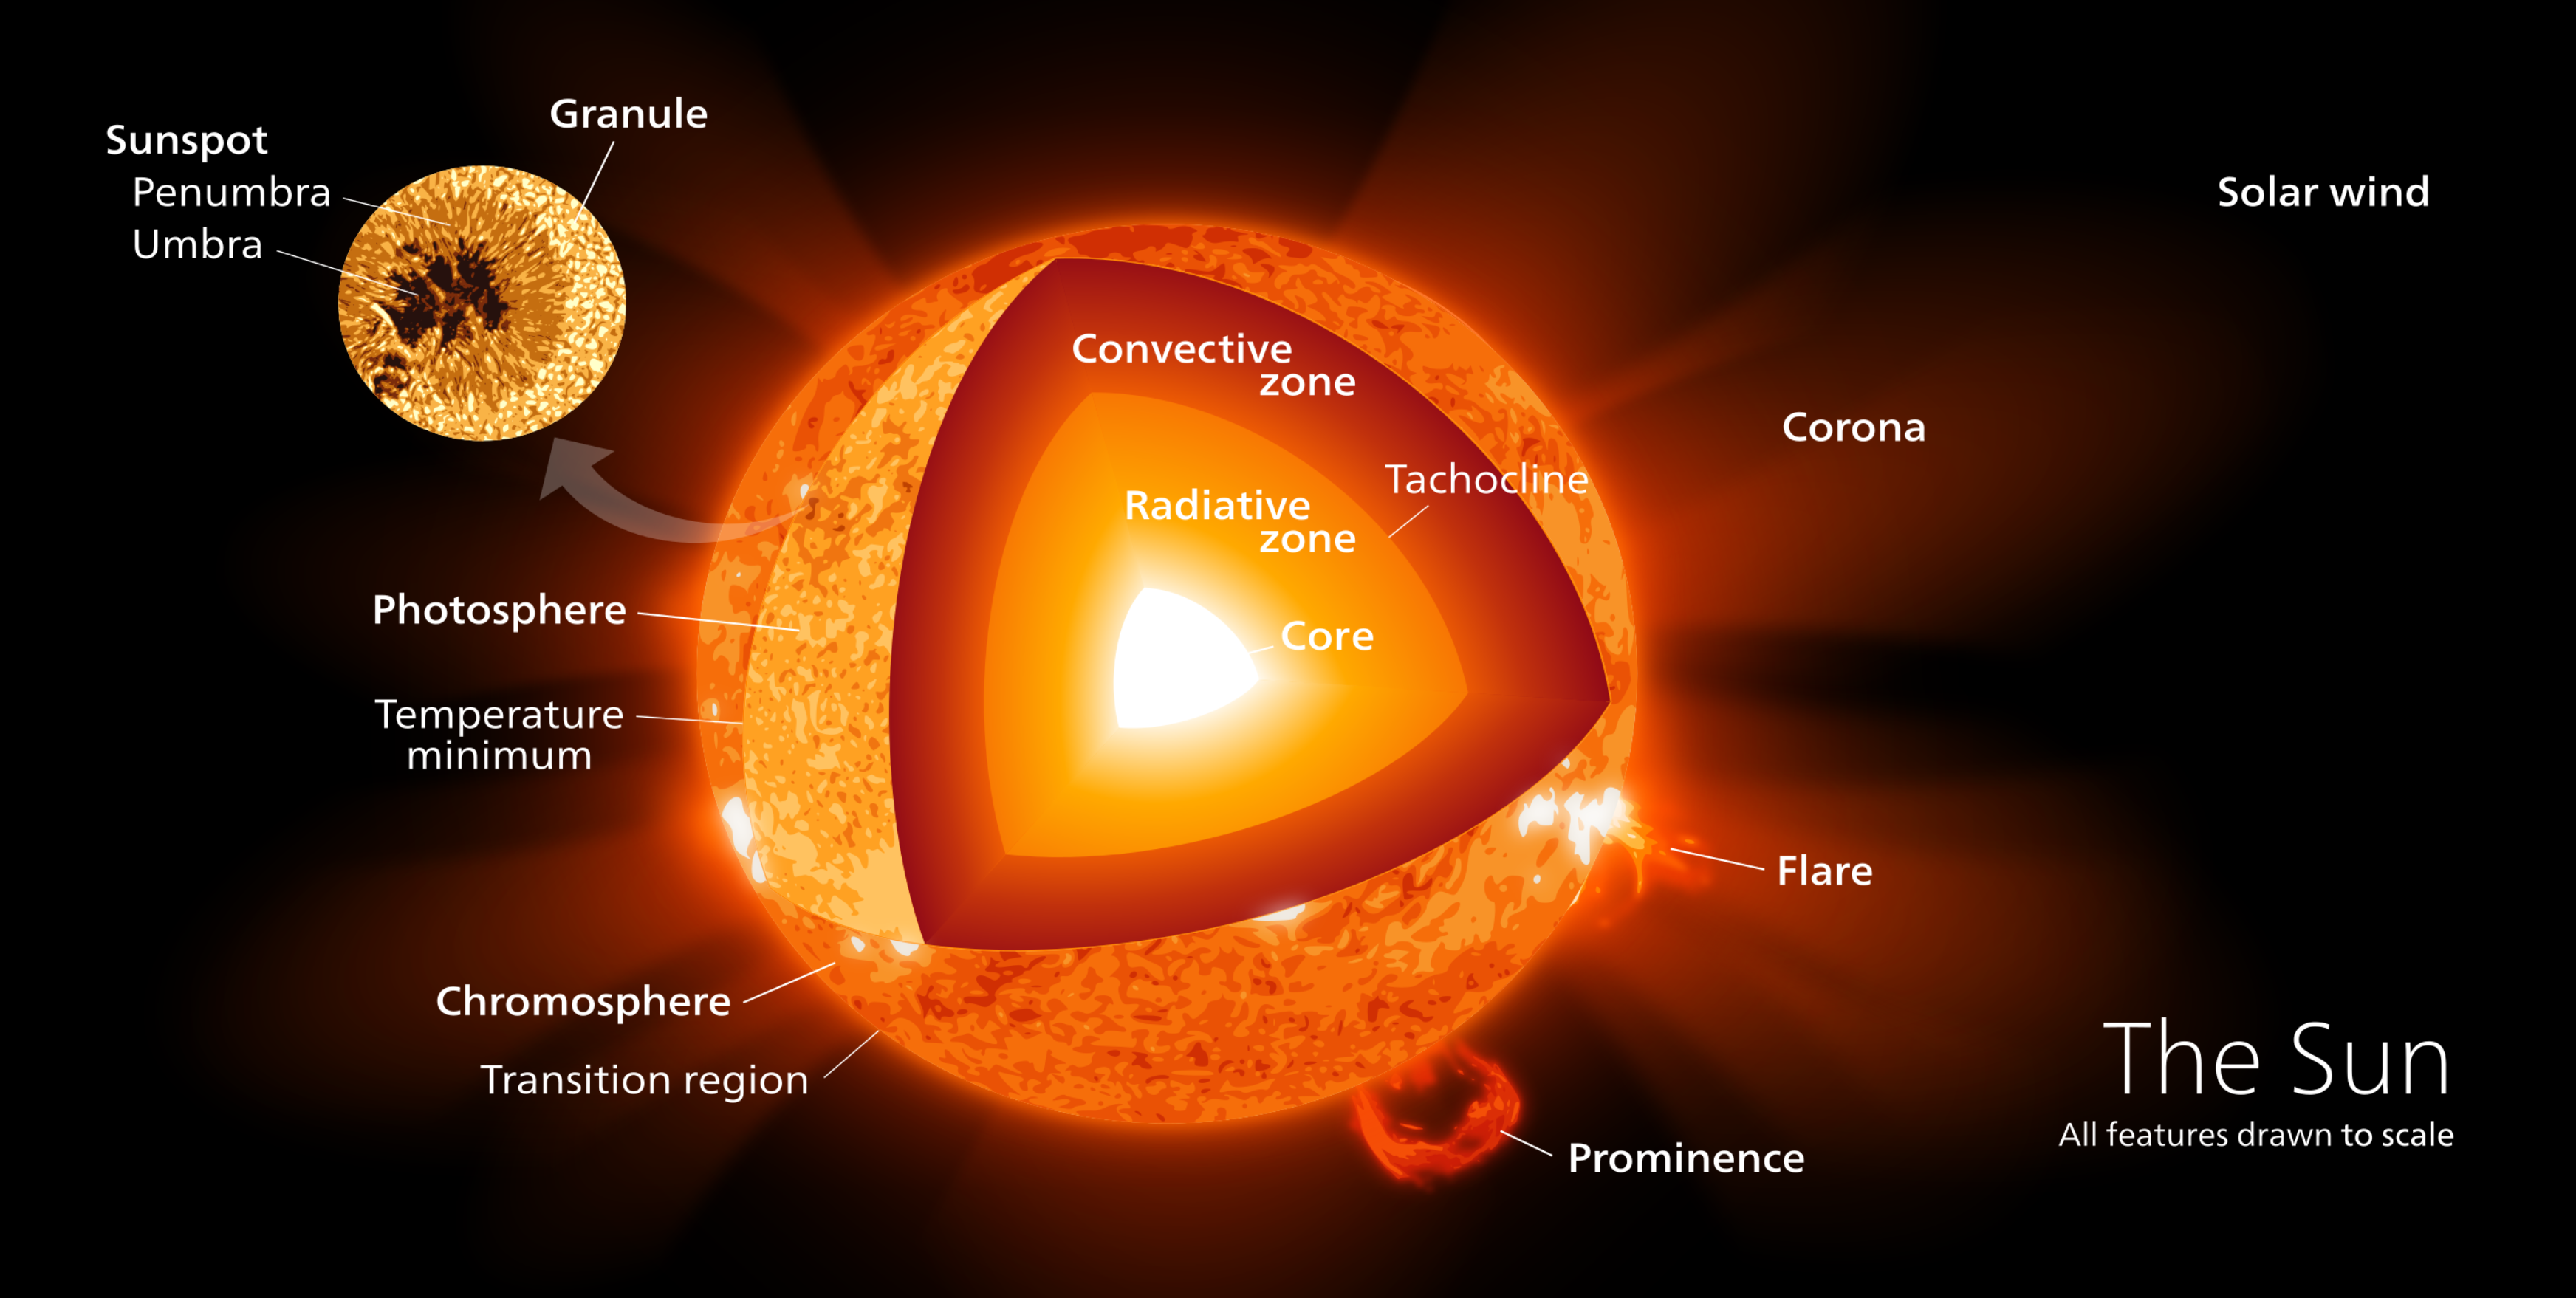
\includegraphics[width=\textwidth]{./pictures/interior.PNG}
    \caption{Visualization of the interior structure of the Sun. \cite{kelvin13}}
    \label{fig:structure}
\end{figure}
In this work we will mainly focus on phenomena related to convection, hence occurring in the convective zone and impacting photosphere.\\
Convection is the transfer of heat from one place to another by the movement of fluids. In particular, regarding the Sun, the temperature at the bottom of the convection zone is 200,000\degree K while at its outermost limit (surface of the Sun) it is being cooled by the creation of light and temperature is only about 5,700\degree K. This large difference triggers the plasma movement in order to propagate the heat outwards. Note, for instance, in Figure~\ref{fig:convect-cells} the bright regions correspond to hot rising material, whereas the dark lanes are the location where the colder material falls down into the Sun \cite{convect}. Also, as the reader can verify from Figure~\ref{fig:convect-cells}, the way convection cells organise on the surface is not regular but rather chaotic and turbulent.
\begin{figure}[t]
    \centering
    \begin{subfigure}[b]{0.49\textwidth}
        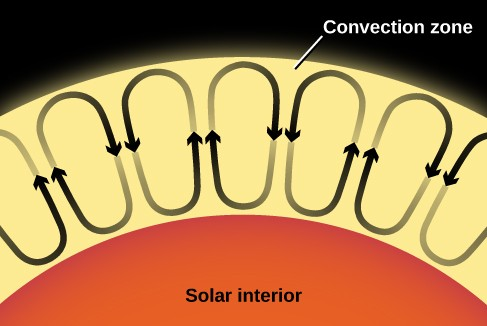
\includegraphics[width=\textwidth]{./pictures/convection}
        \caption{Section view, plasma movement}
        \label{fig:convect}
    \end{subfigure}
    \begin{subfigure}[b]{0.49\textwidth}
        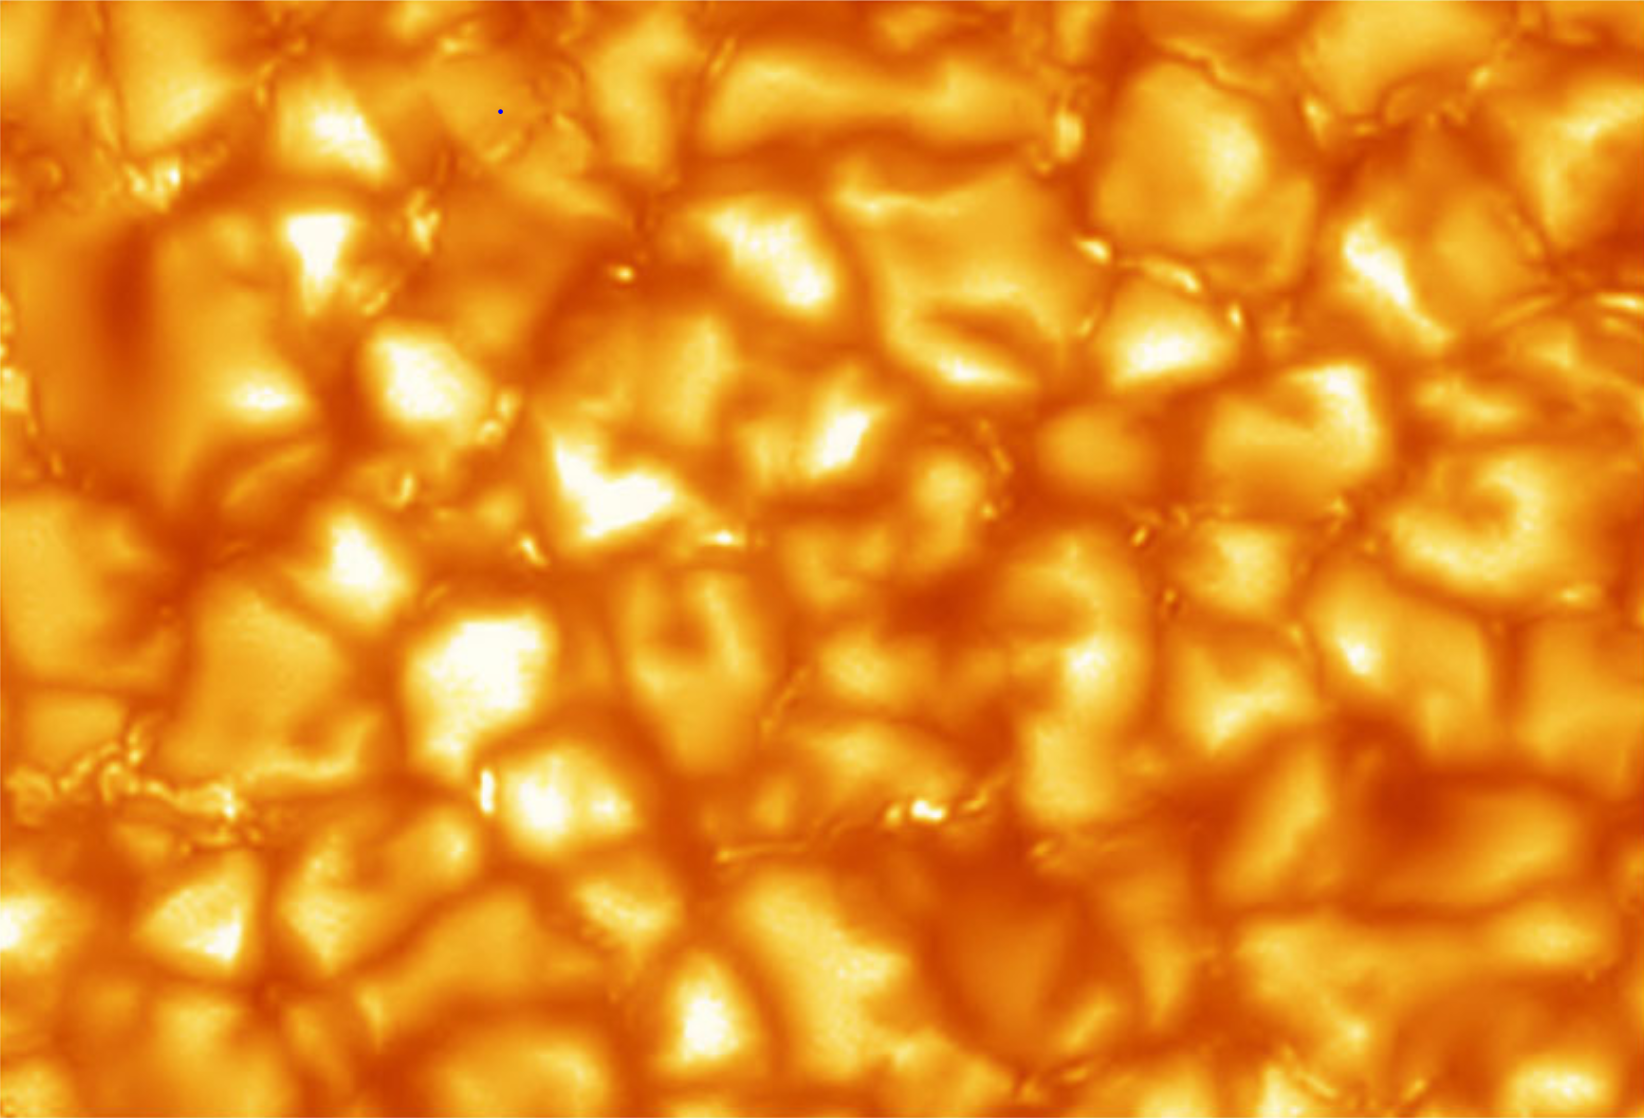
\includegraphics[width=\textwidth]{./pictures/convection-cell}
        \caption{Frontal view, convection cells.}
        \label{fig:convect-cells}
    \end{subfigure}
    \caption{Convection}\label{fig:systemview}
\end{figure}

\begin{figure}[b]
    \centering
    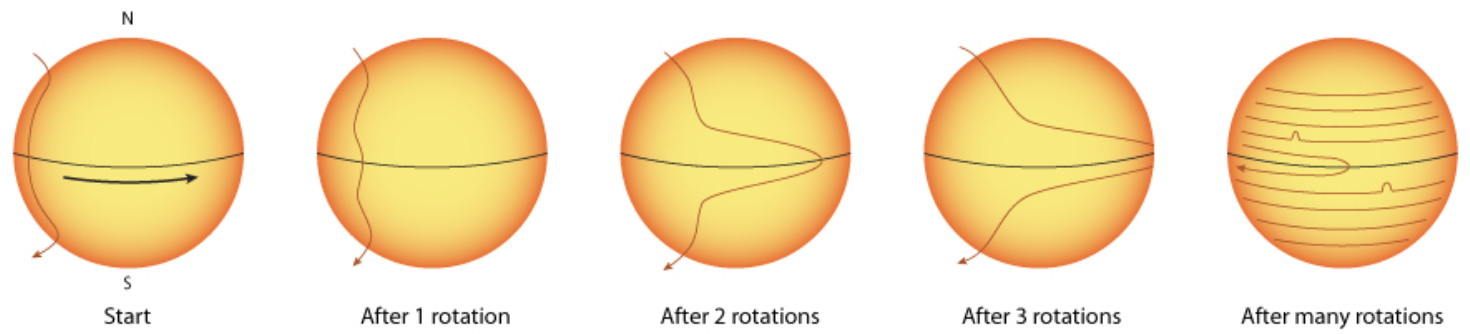
\includegraphics[width=\textwidth]{./pictures/diffrot}
    \caption{Visualization of differential rotation}
    \label{fig:diffrot}
\end{figure}
\begin{figure}[t]
    \centering
    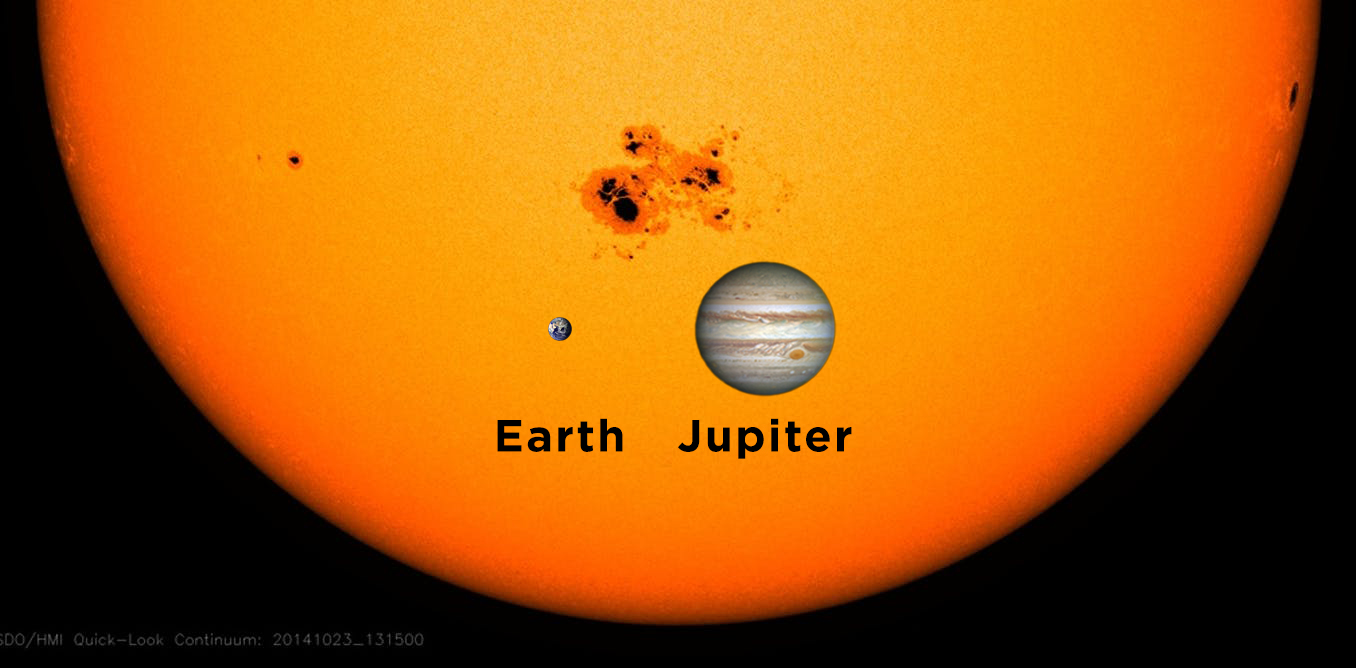
\includegraphics[width=\textwidth]{./pictures/AR12192-jup-earth}
    \caption{Relative size of AR12192, the Earth and Jupiter}
    \label{fig:AR12192-comp}
\end{figure}
Another interesting feature of the dynamics of the Sun is its rotation. In fact the Sun does not rotate uniformly, since it is not a rigid object (a solid body in which deformation is zero or very small). Our star is composed of gasses in the form of plasma and therefore the relative movement of its inner particles cannot be neglected. This results in a type of motion called differential rotation. It has been observed that the angular velocity of the particles changes in a way that depends on the latitude, in particular it is fastest on the solar equator and decreases as latitude increases \cite{diffrot}. From this notion follows that the rotation period is not constant, it takes 24.47 days at the equator and almost 38 days at the poles \cite{diffrotrev}. Furthermore this behaviour has a critical importance for the understanding of this work for two reasons. First, the features that we studied are located on the photosphere and move with the surface of the Sun, undergoing significant deformation. Second, differential rotation together with convective turbulent motions leads to the generation of electric currents and solar magnetic field. This phenomenon is called solar dynamo and is in some way similar to the dynamo effect that generates the magnetic field of the Earth. Moreover the generated magnetic field has the property that it tends to agglomerate into bundles called magnetic flux tubes. When these tubes become strong enough to locally inhibit convection the heat coming from inside the Sun is not propagated upwards and the temperature of the surface decreases significantly. The local temperature drop makes the affected area look darker than the rest of the disk. These black patches, commonly named \textbf{sunspots}, can become very large and thus fairly easy to observe, even with amateur instrumentation. Their average size is comparable to the one of the Earth, but in some cases, when the magnetic perturbation is very strong, they can reach approximately the size of Jupiter or even more, as in the case of AR12192 (Figure~\ref{fig:AR12192-comp}), the largest group of the last solar cycle. As shown in the figure the intensity gap is not uniform, the darkest areas (\textit{umbrae}) locate where the magnetic field is perpendicular to the surface, while on the periphery of the magnetic tube the field is slightly inclined and results in a lighter color (\textit{penumbrae}). Also, it has been shown that, since they indicate intense magnetic activity, sunspots accompany secondary phenomena such as coronal loops, prominences, flares and coronal mass ejections. For this reasons they have been widely observered and studied during the last 400 years. Since the invention of the telescope \cite{king2003history} (early XVII Century) many astronomers started to notice these dark features, although they weren't quite sure about their causes. Some thought they were shadows of undiscovered planets crossing the Sun, while others believed them to be dark clouds in the Sun's atmosphere. In 1843 an amateur German astronomer named Samuel Schwabe discovered the rise and fall of yearly sunspot counts we now call the solar cycle \cite{schwabe1843solar}. Nowadays we actually know that, more in general, the solar cycle is the nearly periodic 11-year change in the Sun's activity that encompasses a multitude of phenomena, as, for example, the variable levels of solar radiation and ejection of solar material. As already discussed, the change in magnitude of the activity of our star is also visible on the Earth; for instance large geomagnetic storms leading to auroras are most common during the peak of the cycle. Soon after the discovery, in 1848, Rudolf Wolf established a relative sunspot number formulation to compare the work of different astronomers using varying equipment and methodologies, known as the Wolf (or Z\"{u}rich) sunspot number \cite{vaquero2007historical}. Such definition is still in use today and we will see how later in this chapter. Wolf succeeded in reliably reconstructing the variations in sunspot number as far as the 1755--1766 cycle, which has since been known conventionally as \textit{Cycle 1}, with all subsequent cycles numbered consecutively thereafter; at the time of writing (early 2019), we are in the final phase of \textit{Cycle 24}, although the first sunspot of \textit{Cycle 25} may have appeared in early April 2018 \cite{cycle25-1}\cite{cycle25-2} or even December 2016 \cite{cycle25-3}. Using Figure~\ref{fig:SILSO2} and Figure~\ref{fig:ssarea} the reader himself can verify that the trend is indeed periodic. The graphics exhibits peaks and valleys; a peak in the sunspot count is referred to as a time of \textit{solar maximum}, whereas a valley, a period when just few sunspots appear is called a \textit{solar minimum}.
\begin{figure}[t]
    \centering
    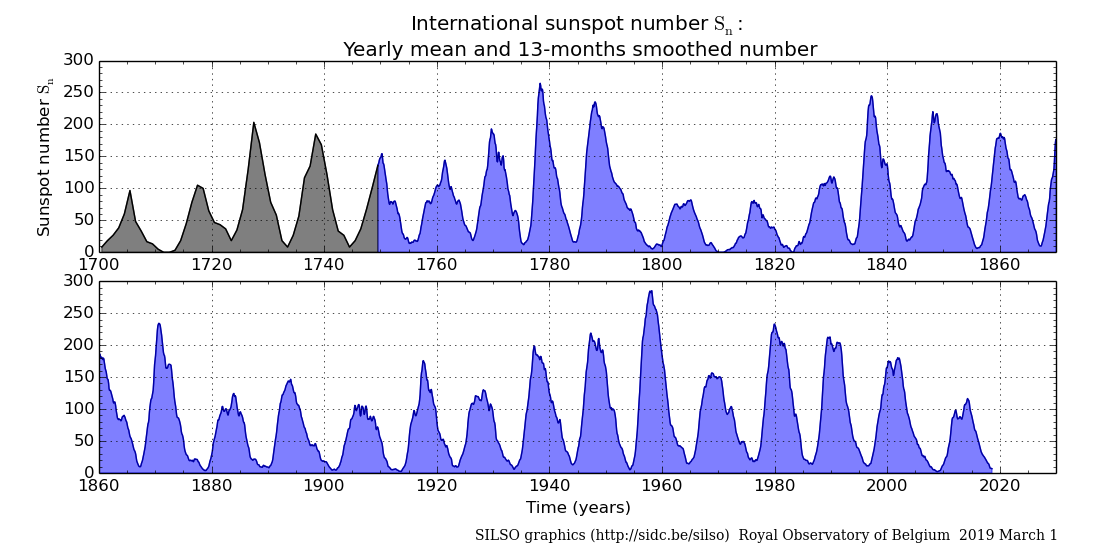
\includegraphics[width=\textwidth]{./pictures/SILSO2}
    \caption{Yearly mean sunspot number (black) up to 1749 and monthly 13-month smoothed sunspot number (blue) from 1749 up to the present.\cite{silso-graph}}
    \label{fig:SILSO2}
\end{figure}
Focusing on Figure~\ref{fig:butterfly} instead, we can discover one more property of the sunspot cycle: \textit{Sp\"{o}rer's law} \cite{ivanov2014sporer}. Sp\"{o}rer's law predicts the variation of sunspot position during a cycle by introducing the concept of \textit{cycle latitude phase} (CLP), that is calculated from the average latitudes of each sunspot over a period of time. It turns out that sunspots tend to appear around 30\degree  to 45\degree  latitude on the Sun's surface. As the cycle progresses, sunspots appear at lower and lower latitudes, until they average 15\degree  at solar maximum. The average latitude of sunspots then continues to decrease, down to about less than 10\degree  and then while the old sunspot cycle fades, sunspots of the new cycle start appearing at high latitudes. The reason why this happens is still not completely understood by the scientists.
\begin{figure}[t]
    \centering
    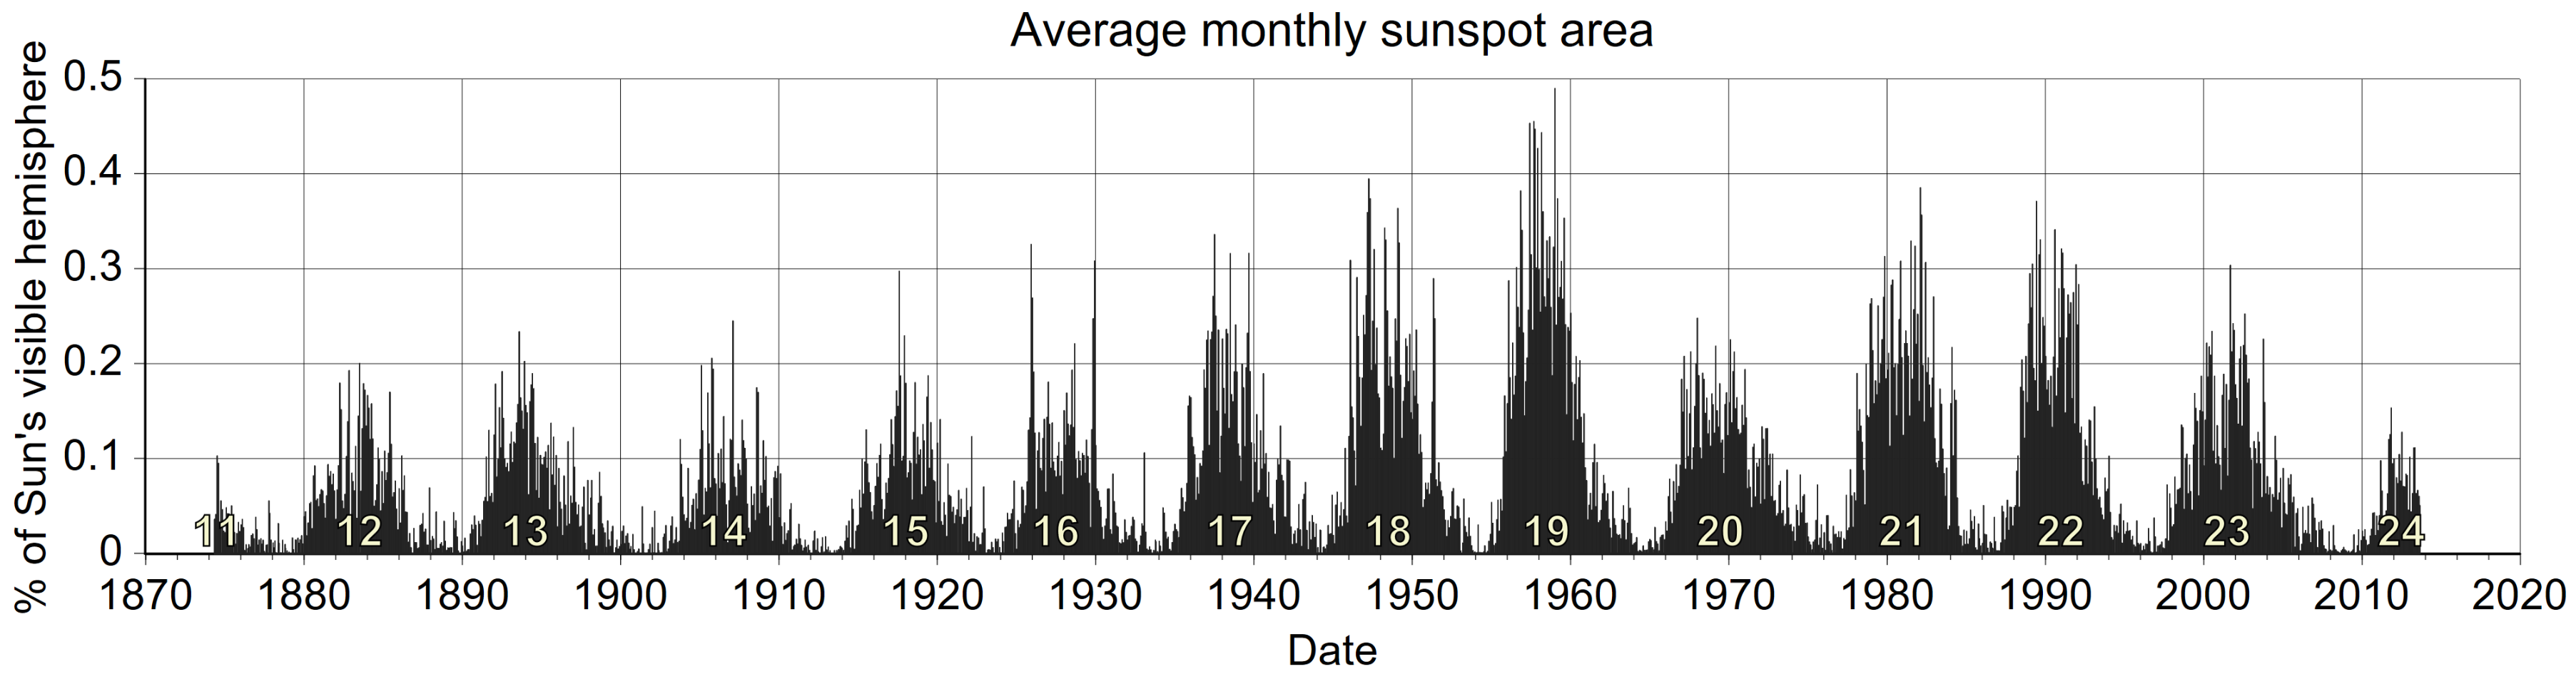
\includegraphics[width=\textwidth]{./pictures/ssarea}
    \caption{Diagram showing average monthly sunspot area from cycle 12 to cycle 24}
    \label{fig:ssarea}
\end{figure}
\begin{figure}[t]
    \centering
    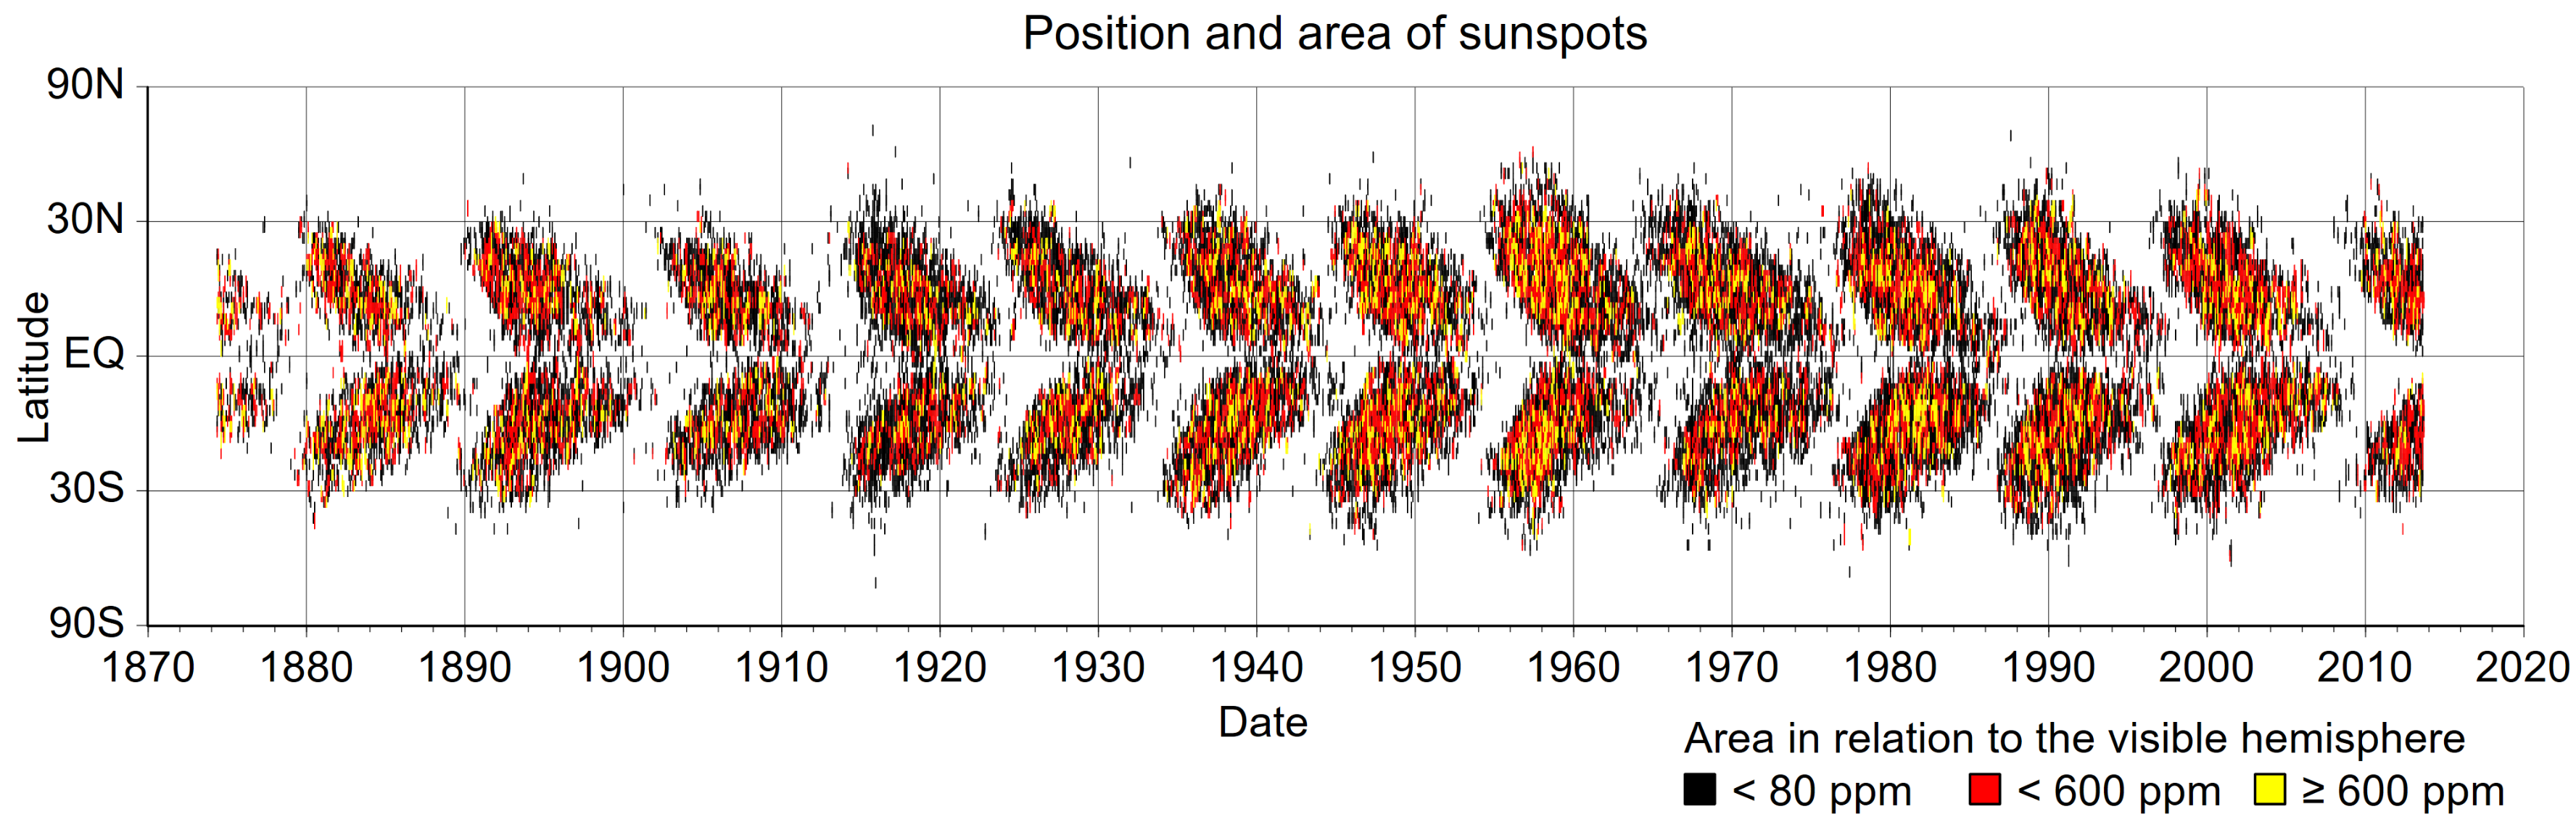
\includegraphics[width=\textwidth]{./pictures/butterfly}
    \caption{Butterfly diagram showing paired position and area of sunspots}
    \label{fig:butterfly}
\end{figure}
Another notion we need to introduce in order for the reader to fully understand this work is sunspot group classification. Several different categorization paradigms have appeared during the years but the one that is most popular nowadays is the \textit{McIntosh classification}, introduced in 1990 \cite{mcintosh1990classification}. The McIntosh classification is constituted by three components, in which the nomenclature used for each sunspot group type is \textbf{Zpc}, where Z corresponds to the \textit{Modified Z\"{u}rich Classification} and the other two components, p and c, reflect the main sunspot characteristics: the type, size, and symmetry of the penumbra and umbra; and the degree of compactness of the group \cite{carrasco2015equivalence}. We will focus on the \textbf{Z} component, that partitions the groups in the following categories\cite{silso-class}:
\begin{itemize}
  \item \textbf{A}: a small single unipolar sunspot. Representing either the formative or final stage of evolution;
  \item \textbf{B}: a bipolar sunspot group with no penumbra on any of the spots;
  \item \textbf{C}: a bipolar sunspot group. One sunspot must have penumbra;
  \item \textbf{D}: a bipolar sunspot group with penumbra on both ends of the group. Longitudinal extent does not exceed 10\degree;
  \item \textbf{E}: a bipolar sunspot group with penumbra on both ends. Longitudinal extent exceeds 10\degree  but not 15\degree;
  \item \textbf{F}: an elongated bipolar sunspot group with penumbra on both ends. Longitudinal extent of penumbra exceeds 15\degree;
  \item \textbf{H}: a unipolar sunspot group with penumbra.
\end{itemize}
Example images for each and every one of the classes can be found in Appendix B.\\
As already described, sunspots and therefore groups are highly correlated with perturbations of the magnetic field of the Sun. In fact, besides being physically close to each other, sunspots belonging to the same groups are usually manifestations of the same \textit{active region}. These are areas of intense magnetic activity that can sometimes cause solar flares and coronal mass ejections. They are observable in several different bands of the spectrum emitted by the Sun, though normally detected using the high-energy ultraviolet band or line-of-sight (LOS) magnetograms. In general, there is a lot of research going on in multi-wavelength solar analysis, that is the field that investigates the Sun interpolating knowledge among different wavelengths. These studies are also pushed forward by the modern instrumentation we possess. Nowadays spotting active regions is pretty easy and can be achieved with several different tools (refer to Chapter 2 for more information). Once every active region is recognised it is fairly easy to determine which sunspot belongs to which group. Still, the notion of sunspot group was born a long time before active regions were observed for the first time. To clarify this, it is sufficient to think that the relationship between sunspots and magnetic field is a relatively recent finding and magnetographs only appeared at the beginning of 20th Century. However this doesn't mean that all the studies that were carried out before the invention of sophisticated space telescopes should be dismissed as ``outdated''. The complexity of modern instrumentation makes their lifespan limited and the dataset they produce quite unique. On the contrary, ground-based observatories have been pointing at the Sun during more than 400 years making it one of the longest scientific experiment in the human history. Longevity makes it possible to capture secular variability and therefore enabling long-term analysis that wouldn't be possible otherwise. Sure enough, ground observation has its own limitations as well. Despite being very stable in the long term it can't be considered reliable in short periods of time. In fact, considering a single observatory as source of data, it is impossible to estimate the daily number of sunspots consistently. This happens because the quality of the data is strongly affected by the dynamics of the atmosphere. If the thick layer of air that sits inbetween the telescope and the Sun is turbulent or hazy the resulting images will loose definition, intruducing a bias on the sunspot count. On the other hand, if the atmosphere is quiet and transparent the light will travel without trouble, making the obseravtions almost as good as the ones of space telescopes. It is understood that if the solar disk is obscured by the clouds during the whole day the counting is impossible and it should be regarded as a missing data point. Nowadays, to overcome these limitations the SIDC/SILSO \cite{sidc-silso}, the most important authority in the field, uses an ensemble of hundreds of observatories to produce the sunspot number series \cite{Clette2015}. Averaging over several heterogeneous detections has many benefits, namely: mitigating the variance, improving accuracy and solving missing data problems. However, it also introduces a new layer of complexity in the computation of the final index, since it is not possible to perform a simple average considering that the available stations are different from day to day. Every set-up has its own, unique properties that should be taken into account in the calculation. Luckily, this uniqueness is already captured in the personal reduction coefficient ($K$) included in the \textit{relative sunspot number} formula by R. Wolf:
\begin{equation}\label{relssnum}
R = K \cdot (10 \cdot g + s)
\end{equation}
The way this solar activity index is calculated hasn't changed much since its establishment, 400 years ago. What changed, though, is our ability to resolve very small spots on the surface of the Sun and highlight them through post-processing. \\
An example of the processing techniques that can help scientists in the counting is \textit{limb darkening correction}. This method consists in the reduction of the phenomenon of limb darkening through software. This phenomenon is an optical effect intrinsic to the physics of the observation, that causes an imbalance in the quantity of photons we receive from the limb of the disk compared to its center (refer to Figure~\ref{fig:AR12192-comp} for a visual intuition). In practice, this can be pleasant to the eye because it gives the viewer the idea of the sphericity of the Sun, but it is also inconvenient when trying to detect small features on the edge. The theoretical laws that govern the magnitude of the darkening for each point of the surface are very rich and interesting but they are out of the scope of this thesis. In any case, there are much simpler solutions that are able to correct the images only leveraging the intensity profile of the image (more details will be given in Chapter 3). Other interesting post-processing techniques for feature enhancement will be illustrated in Appendix C, including for instance gradient sharpening, off-limb emission enhancement and mean intensity correction. \\
Finally, to conclude this brief introduction to solar physics, it is necessary to present some basic aspects of the large topic of \textit{solar coordinate systems}. Standardizing the way the position of solar features is encoded is vital for the creation of large scale datasets, but at the same time it is very difficult for several reason. The first reason is that the axis of rotation of our star is tilted with respect to the ecliptic of the Earth. Therefore the solar north pole, as seen from the our planet, appears displaced. Clearly, the displacement is not constant, but rather periodic. As the Earth procedes on its orbital path, the observed axial tilt changes in a range that goes from -7\degree to 7\degree. The second reason that should be considered in the study of solar coordinates is that the Sun is a gaseous body, there are no fixed points of reference and this is made worse by differential rotation. Moreover it is also not perfectly spherical, although its oblateness is rather small and almost neglectable \cite{dicke1974oblateness}. The last reason is represented by the fact that the revolution and rotation of the Earth itself influences our perspective of the Sun. For this reason, a coordinate should not really be considered complete if it doesn't include time. The deveopment of sophisticated coordinate systems for solar image data allows to overcome, at least partially, these difficulties. Nowadays, solar coordinate systems can be divided into 3 categories \cite{thompson2006coordinate}:
\begin{enumerate}
  \item \textbf{Heliographic Coordinates}: latitude and longitude of a feature are expressed on the solar surface, and can be extended to three dimensions by adding the radial distance from the center of the Sun. There are two basic variations on the heliographic system: \textbf{Stonyhurst} and \textbf{Carrington} heliographic. Both use the same solar rotational axis (based on the original work by R. Carrington in 1863), and differ only by an offset in the longitude definition.
  \item \textbf{Heliocentric Coordinates}: any system of coordinates where the origin of the axes is located at the centre of the Sun. The system can be \textbf{cartesian}, when the z axis is defined to be parallel to the observer-Sun line and the y axis points towards the north pole, or \textbf{radial} if it uses a position angle measured from the projection of the north pole and a radial distance.
  \item \textbf{Helioprojective Coordinates}: observations are projected against the celestial sphere and all projective angles have origin at disk center, considered as the apparent disk center as seen by the observer without any corrections made for light travel time or aberrations.
\end{enumerate}



% \begin{figure}[b]
%     \centering
%     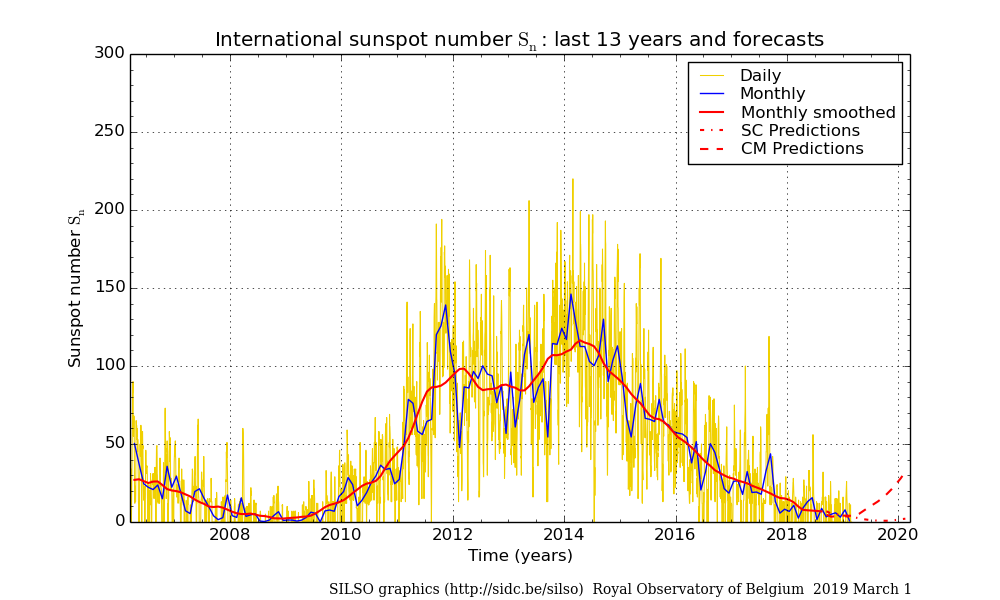
\includegraphics[width=\textwidth]{./pictures/SILSO1}
%     \caption{Daily sunspot number (yellow), monthly mean sunspot number (blue), smoothed monthly sunspot number (red) for the last 13 years and 12-month ahead predictions of the monthly smoothed sunspot number. SC = prediction method based on an interpolation of Waldmeier's standard curves. CM = method (from K. Denkmayr and P. Cugnon) combining a regression technique applied to the sunspot number series with the a geomagnetic index used as a precursor}
%     \label{fig:SILSO1}
% \end{figure}
%
%
% \begin{figure}[t]
%     \centering
%     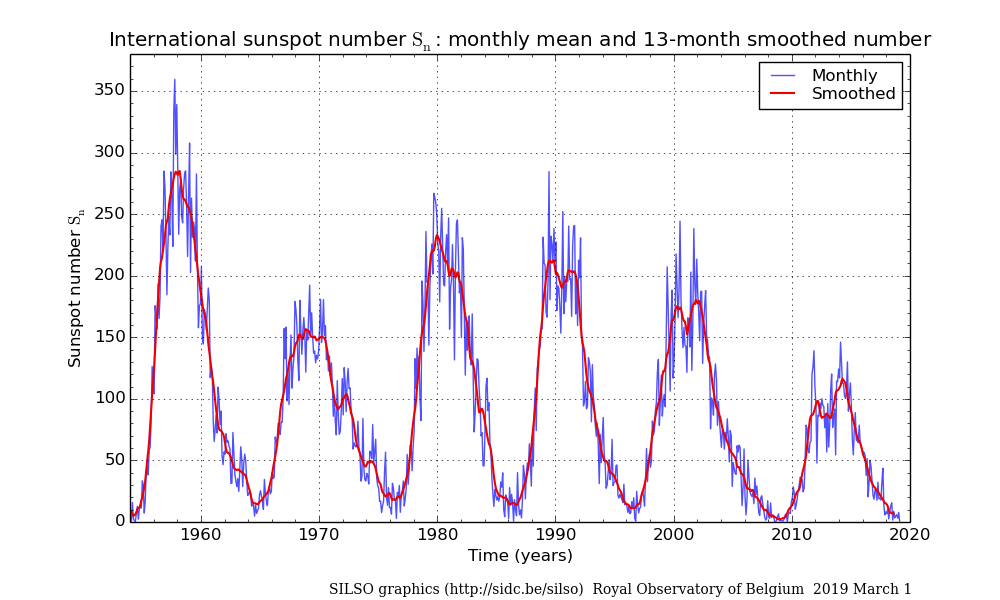
\includegraphics[width=\textwidth]{./pictures/SILSO3}
%     \caption{The monthly mean sunspot number (blue) and 13-month smoothed monthly sunspot number (red) for the last five cycles.}
%     \label{fig:SILSO3}
% \end{figure}

% \begin{figure}[t]
%     \centering
%     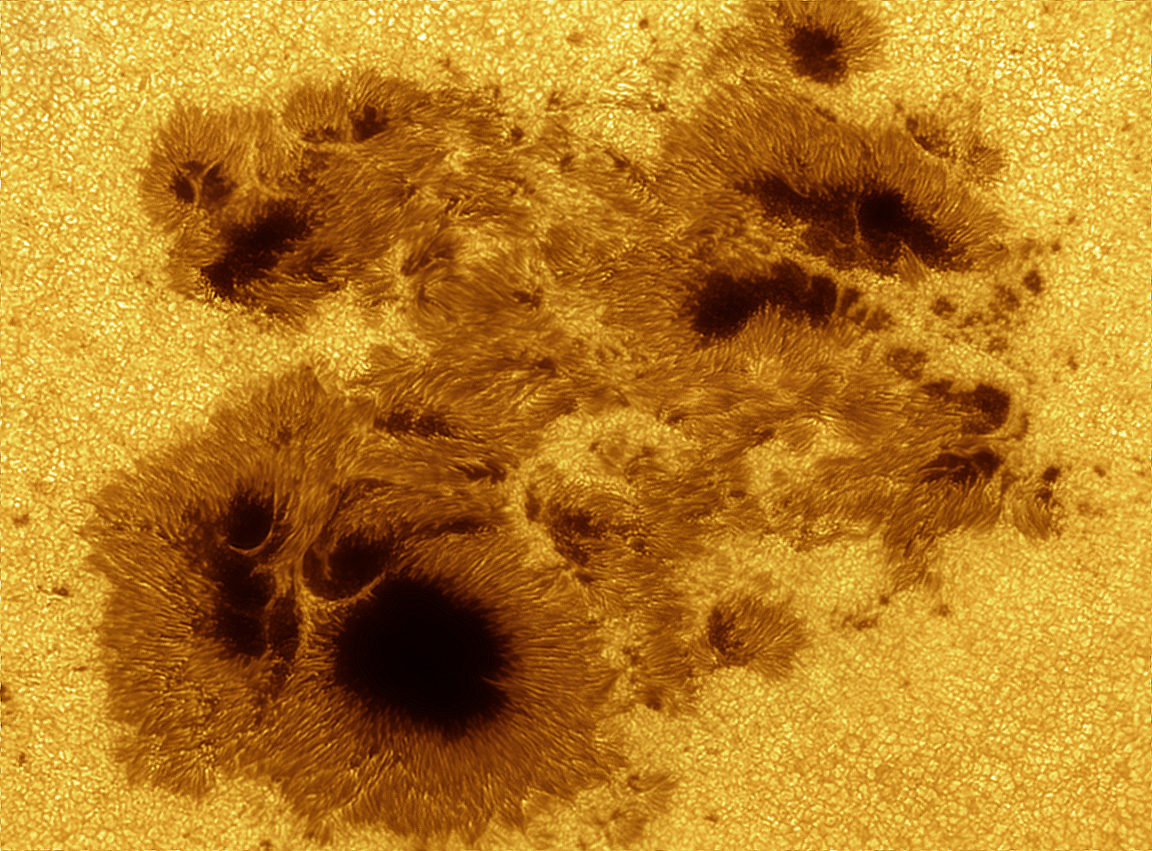
\includegraphics[width=\textwidth]{./pictures/AR12192}
%     \caption{Close up picture of AR12192}
%     \label{fig:AR12192}
% \end{figure}

\chapter{Impostazione del problema di ricerca}
\label{capitolo3}
\thispagestyle{empty}
\chapter{Progetto logico della soluzione del problema}
\label{capitolo4}
\thispagestyle{empty}

\chapter{Problem Statement}
\label{capitolo5}
\thispagestyle{empty}
\noindent The amount of magnetic flux that rises up to the Sun's surface varies with the progress of the solar cycle. Visible sunspots on the disk are one of the manifestations of the perturbations of the magnetic field. The inner activity of the star and the flow of particles that get blasted out from the outer layers also depend on the intensity of these perturbations. It follows that, improving our estimate of the sunspot index would also make our space weather predictions more reliable. One could think that determining the sunspot count univocally could be possible. Unfortunately, it turns out that, for several reasons, it is not possible. The personal reduction coefficient $K$ in the relative sunspot number formula \eqref{relssnum} tries to mitigate this exact problem. It captures both the variability due to the observation and the subjectivity of the observer. Ideally, if the person in charge of manually counting and grouping sunspots was the same in all the observatories of the world, then the variance generated by subjectivity would be neglectable. This is clearly not possible. But imagine having an algorithm that can learn from the experts and be distributed and run by every observatory. This would guardantee constant detection standards if the parameters of the program were identical in all the stations. So far, the automatic methods that have been proposed show two main problems: first, they are not general, so they cannot be used on heterogeneous data without retuning the parameters; second, they are not reliable enough to work without human supervision. These drawbacks basically break the hypothesis that the algorithm is indeed consistent in the estimation of the number of sunspots. This happens because those methods are not based on the understanding of the scene, but rather they leverage very specific properties of the data. Advanced computer vision algorithms, instead, focus on the semantic of the image, making assumptions on the data much less important. This thesis proposes a deep learning approach to sunspot counting and aims to be a step forward in the integration of computer vision into solar physics.\\
Before diving deep into the practical details of this work, we need to define the problem in a more formal way. Basically, the only theoretical physics device that will be used is the relative sunspot number formula \eqref{relssnum} that will be shown here again for the sake of clarity:
\begin{equation}
  R = K \cdot (10 \cdot g + s)
\end{equation}
Therefore, the three variables that we will need to be able to calculate are:
\begin{itemize}
  \item the number of sunspots $s$;
  \item the number of groups $g$;
  \item the personal reduction coefficient $K$ of the algorithm.
\end{itemize}
\begin{figure}[b!]
    \centering
    \captionsetup{justification=centering}
    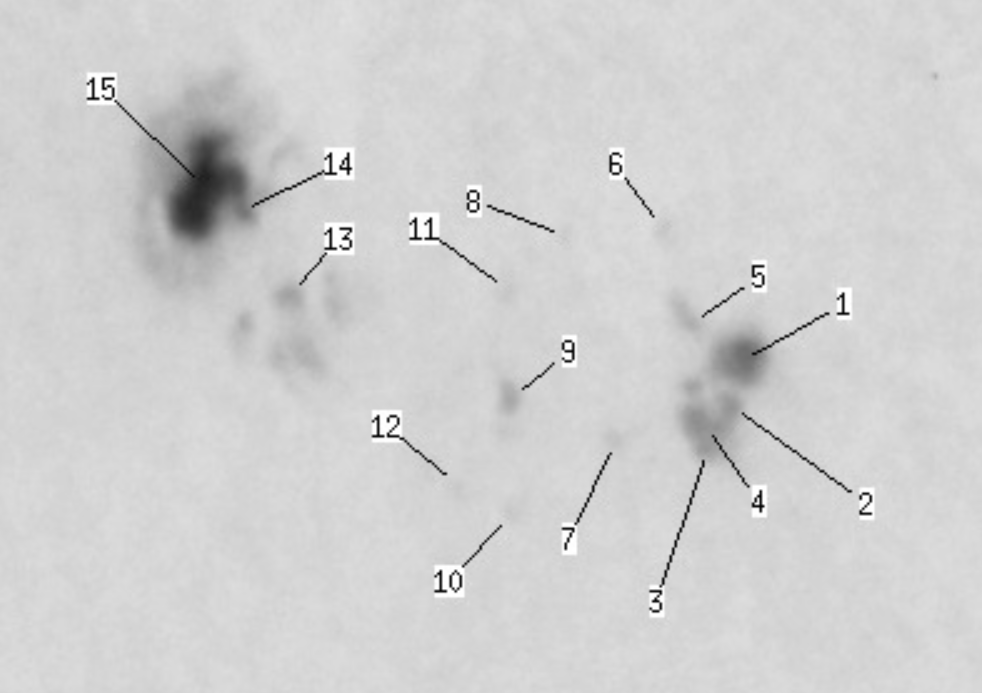
\includegraphics[width=\textwidth]{./pictures/sunspot-annotation}
    \caption{Annotated group of sunspots.}
    \label{fig:sunspot-annotation}
\end{figure}
The identification of each one of these variables carries its own challenges. In Figure~\ref{fig:sunspot-annotation} the reader can appreciate a manual annotation of a group of sunspots by an expert scientist. Each label refers to a single sunspot so the total number of sunspots in the image is equal to the number of labels that are present. Note that the annotation is not as straightforward as it seems, for example label \text{13} refers to more than one dark area while labels \textit{2, 3, 4} all map to a single black spot. We won't go into detail about why labels have been assigned this way but the reader can assume that the expert annotator has a deep understanding of the behaviour of the magnetic field and therefore he is able to distinguish real sunspot instances from artifacts. In the case of Figure~\ref{fig:sunspot-annotation} the sunspot group was found near the center of the disk, but there are cases where the sunspots appear much closer to the limb. In those cases the viewing angles are very high and the annotation is a lot harder, because of
perspective deformations and the limb darkening effect.\\
Once all the sunspots in the image have been annotated they can be clustered into groups. Again, in Figure~\ref{fig:annotated-mask} the reader can get an impression of what it means to find sunspot groups. If the magnetogram of the solar disk is available, it is fairly easy to detect active regions first, and then map each sunspot to the closest one. For the reasons that have been explained in Chapter~\autoref{capitolo2} it will be supposed that the magnetogram is not available. So, clustering has to be performed by inferring the magnetic link between each sunspot. Sunspot classification can be used as an aid for clustering. In fact, broadly determining the class while forming a group is important to make sure that the magnetic properties are respected. Nevertheless, when the cycle is near to the peak active regions tend to be very close to each other. This behaviour is showed in Figure~\ref{fig:annotated-mask}, where groups 11516 (grey) and 11517 (red) are almost overlapping. In such a situation separating or not the two groups is a rather subjective matter that causes inconsistecies.\\
Finally, the personal reduction coefficient is usually estimated statistically. Since sunspot counting is done on a daily basis, $K$ can be recalculated every day taking into account past observations. SILSO implements a similar procedure using a pilot station as a reference, and, for simplicity they recalculate once per month, instead of daily. \clearpage
\begin{figure}[h!]
    \centering
    \captionsetup{justification=centering}
    \begin{subfigure}[t]{0.45\textheight}
        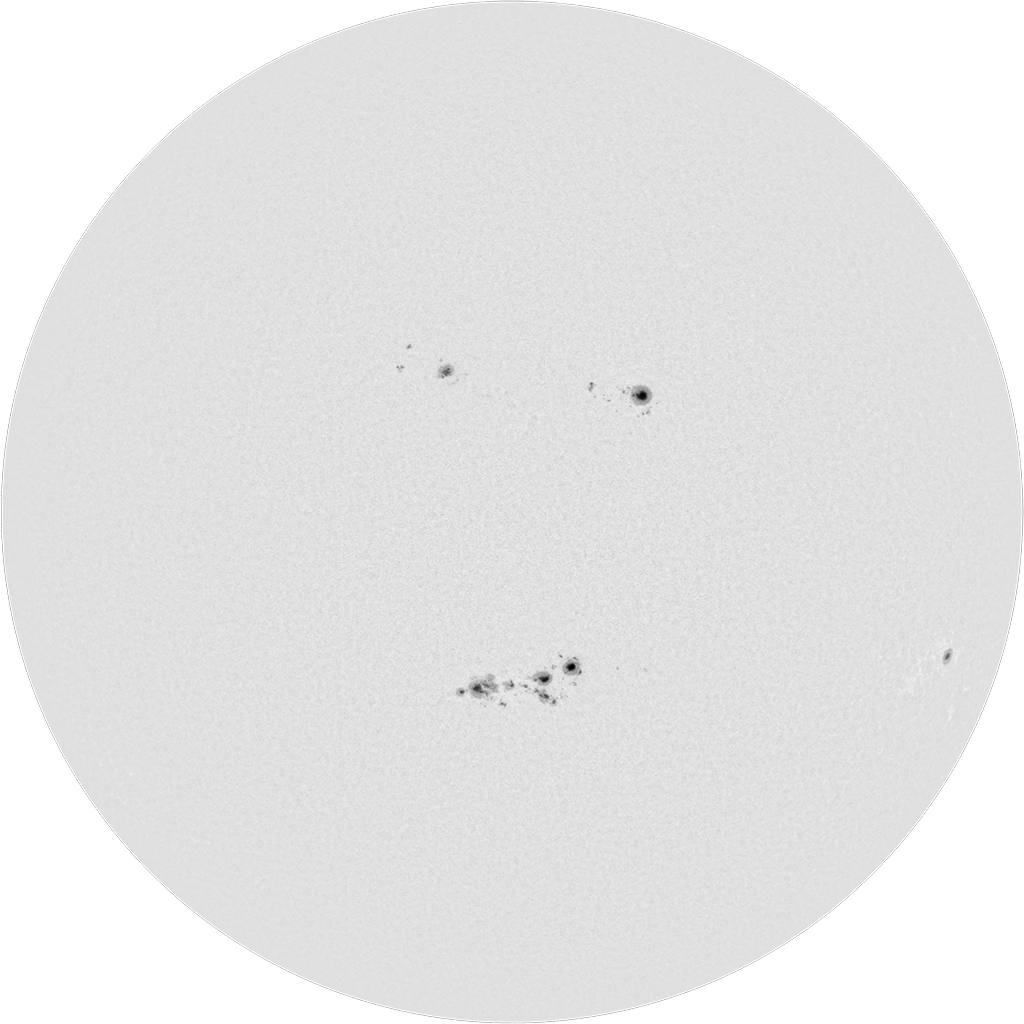
\includegraphics[width=\textwidth]{./pictures/groups-white-light}
    \end{subfigure}\vspace{3mm}
    \begin{subfigure}[t]{0.45\textheight}
        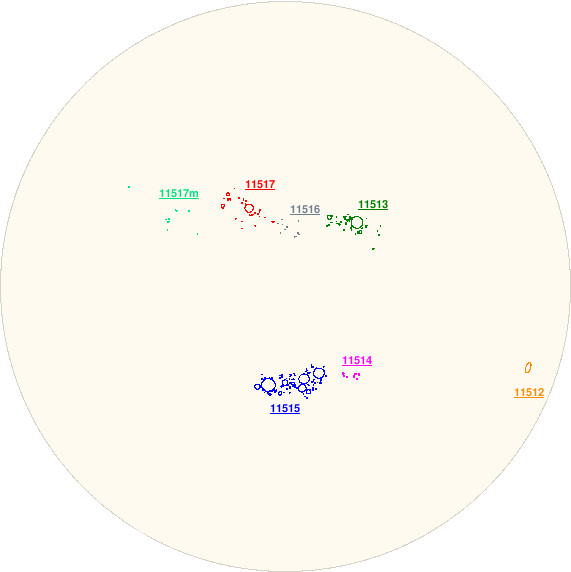
\includegraphics[width=\textwidth]{./pictures/groups-annotation}
    \end{subfigure}
    \caption{Complete solar observation, 03/07/2012. Top: full-disk white-light image, Bottom: annotated mask with colorized sunspot groups}\label{fig:annotated-mask}
\end{figure}

% \chapter{Dataset}
\label{capitolo6}
\thispagestyle{empty}
\noindent The abundance of astronomical data provides great opportunities for machine learning. In fact, most of the data is free to use for anybody and labels are almost always available. Solar physics is no exception to that. Many public databases of solar events can be downloaded in textual form and then annotations can be reconstructed from them. However, the reconstruction is not trivial sometimes, since a good understanding of solar coordinate systems is required.\\
In this work 4 datasets have been merged together:
\begin{itemize}
  \item \textbf{Debrecen Photoheliographic Data (DPD) \cite{baranyi2016line}\cite{gyHori2016comparative}}: a catalogue of positions and areas of sunspots from 1974 until present times, compiled by using white-light full-disk observations taken at the Heliophysical Observatory of the Hungarian Academy of Sciences (Debrecen, Hungary) and its Gyula Observing Station as well as at other observatories;
  \item \textbf{Sunspot Index and Long-term Solar Observations (SIDC-SILSO) Dataset \cite{clette2014revisiting}}: a time series of daily total sunspot number derived with the relative sunspot number formula \eqref{relssnum}, provided by the Royal Observatory of Belgium using a network of observers. This dataset will be used for validation and testing purposes only;
  \item \textbf{Virtual Solar Observatory (VSO) \cite{hill2009virtual}}: a tool for investigating the physics of the Sun, by searching and downloading existing databases for terrestrial and space-based observations;
  \item \textbf{US Air Force, Mount Wilson (USAF/MWL) Dataset}: a catalogue that provides a list of sunspot regions and their parameters, observed by the USAF solar observatories and the Mount Wilson observatory. In particular, it is famous for sunspot group classification data.
\end{itemize}
The last solar cycle was selected as a use case for the training and testing of the algorithm. Both ground and space telescope data were added up to form a quite large dataset. One full-disk observation was considered for each day, drawn and reconstructed from the DPD dataset. Space based data ranging from 2011 to 2014 was downloaded with a Python module called SunPy \cite{mumford2015sunpy} that connects to VSO's open APIs, while ground based data from 2011 to 2013 was obtained directly from DPD's FTP access. Due to availability problems, the ground observations for 2014 were missing from the database. Since the images came from different datasets some pre-processing was necessary to unify them. Ground based observations came in the form fits files with variable resolution (from 4096x4096 to 8192x8192), where limb darkening correction had already been applied but the disk was not centered in the the plate. So, first, the center, radius and axial tilt of the Sun were extracted from the header in order for the Sun to be aligned and cropped from the raw image. The coordinates of the sunspots were given in the DPD dataset in heliocentric-radial coordinates. From those, using simple trigonometry, it was easy to calculate the positions in pixel coordinates.
On the other hand, the preprocessing of space based observations needed a bit more work. For each day, sunpost instances were extracted from DPD, and SDO images were searched inside the VSO using date and time of the DPD observation. The temporally nearest image was selected and downloaded. Despite the fact that SDO observations are very frequent, the average delay between the image and the annotated mask was around half an hour on average. This time shift is pretty large, considering that the Sun rotates and the Earth moves on the orbit (SDO can be considered solidal to the Earth in this case). The misalignment was big enough to make it necessary to rotate the positions of the sunspots to create very accurate masks. Luckily, DPD also provides Carrington heliographic latitude and longitude for each sunspot. These coordinates can easily be transformed into the helioprojective system. At this point, the images were loaded as a SunPy Map, a class that contains many useful methods to interact with solar data. One of these functions allows to calculate where an helioprojective coordinate maps to, after a time delta, taking into account the differential solar rotation profile. This works well when the sunspots are big because the magnetic tubes that create them usually have a lot of ``inertia'', and therefore move pretty consistently with the rotation profile. Marginal misalignments still arise when sunspots are very small, because even a modest change in the magnetic perturbation causes erratic movements, making it difficult to predict their location. After these calculations, it was the turn of limb darkening correction. From the center of the disk, circles of increasing radius are created and the pixels that lay on the border of the circle are averaged, creating the limb darkening profile (blue points in Figure~\ref{fig:sldtk}). A polynomial function is fitted on these data points and then, for every pixel, the right correction is applied to straighten the profile.
\begin{figure}[t]
    \centering
    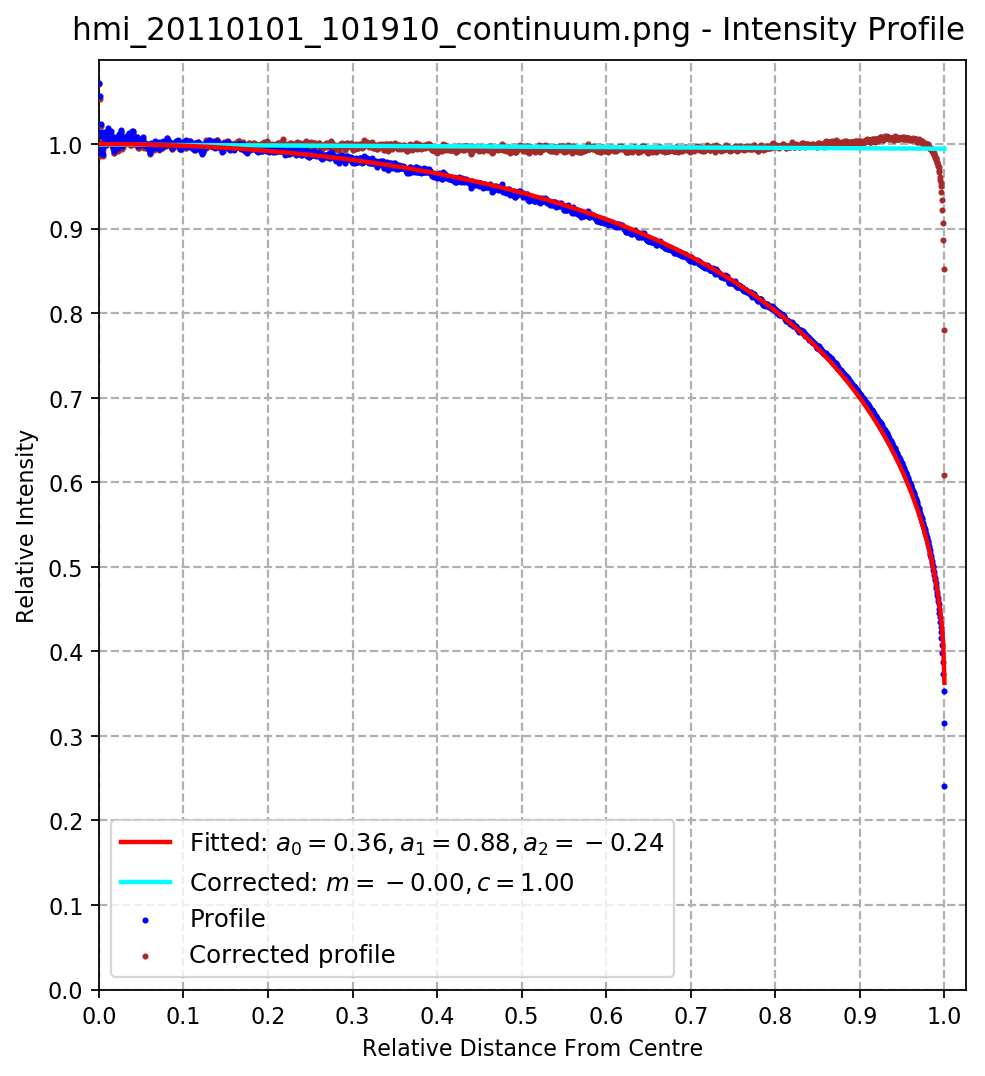
\includegraphics[width=\textwidth]{./pictures/SLDTk}
    \caption{Limb darkening intnsity profile created with SLDTk \cite{sldtk}.}
    \label{fig:sldtk}
\end{figure}\\
Once the coordinates of the sunspots are ready for both ground and space observations, the segmentation masks can be generated by a flooding procedure. For each sunspot a seed is initialized from its coordinates. From the seed, the procedure starts to explore the pixels around it in a breadth first fashion, so that for every iteration the pixels with lowest value are selected for expansion. By doing so, the algorithm floods the darkest areas of the image first, remaining trapped into the penumbra. Using the whole spot area provided by DPD, it is possible to calculte the exact number of pixels of each sunspot and therefore make the expansion stop exactly on the edge of the penumbra. All the pixels that have been selected at least once are then written on a black array that has the same shape of the original image, to create the segmentation mask. Actually, the final mask also contains information about the groups and their classes in order to train the second part of the algorithm. The annotations created by this procedure are consistently good in practice, as it can be appreciated from Figure~\ref{fig:annotated-sunspot}. The figure also shows how the precision of the mask increases with the size of sunspots. For instance, the contours of the small rightmost sunspots are not correctly captured in the mask, while the largest ones are almost perfectly represented.\\
\begin{figure}[t!]
    \centering
    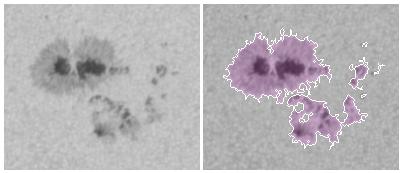
\includegraphics[width=\textwidth]{./pictures/blanquish}
    \caption{Example of a sunspot group mask.}
    \label{fig:annotated-sunspot}
\end{figure}
Overall, data preparation was probably the hardest and most time consuming part of the work, but the results repay the effort. The final analysis on the dataset shows the following statistics:
\begin{itemize}
  \item 2555 images with 4K resolution;
  \item around 21000 sunspot group instances;
  \item around 190000 single sunspots;
\end{itemize}
However, in order to train the algorithm and be able to asses its performance, it is necessary to divide the dataset into three subsets:
\begin{enumerate}
  \item \textbf{training set}: the part of data the algorithm will learn from;
  \item \textbf{validation set}: the sample of data that is used to provide an unbiased evaluation of the model while tuning hyperparameters. In our case the validation set will be particularly useful to estimate the personal reduction coefficient ($k$);
  \item \textbf{test set}: the chunk of data that will be used to estimate the final performance of the model once it is completely trained.
\end{enumerate}
The dataset was split accordingly trying to minimize the dependencies among the subsets. The initial idea was to split the dataset randomly, sampling observations for each month. This would have enabled us to estimate more precisely the average monthly sunspot number in the testing phase, because the observations would have been homogeneously distributed. Unfortunately, this is not a good approach because it introduces strong dependencies in the data, since sunspots can last even more than ten days on the disk and therefore the same sunspot could have appeared in both training and test data. A simple strategy is to divide the dataset while reducing regularities is to sample observations consecutively for the validation and test sets. So for each month the data was partitioned as follows:
\begin{itemize}
  \item days from the 1\textsuperscript{st} to the 19\textsuperscript{th} were assigned to the training set;
  \item days from the 20\textsuperscript{th} to the 24\textsuperscript{th} were assigned to the validation set;
  \item days from the 25\textsuperscript{th} to the last one of the month were assigned to the test set;
\end{itemize}
This data split design doesn't completely solve the dependency problem. In fact, though harder, it is still possible that the same sunspot appears repeated among the three sets. However, the longer the sunspot survives on the disk the more deformation it undergoes, strongly mitigating the dependency issue. Also, this partitioning strategy is a good trade-off because it still enables us to make monthly activity charts, averaging the results over the test set.
\clearpage

% \chapter{The Model}
\label{capitolo7}
\section{Training}
\subsection{Full-Disk Image Segmentation}
\noindent We argued that the problem of estimating the activity of the Sun ultimately reduces to the calculation of the relative sunspot number. A fundamental step for this calculation is finding the number of single sunspots in a full-disk image of the Sun. Semantic segmentation was selected as a tool to identify the areas of the disk that contain a sunspot, intended as all the pixels that fall inside the border of the penumbra, as opposed to the areas where the Sun is quiet.
\bigbreak
\noindent In practice, we need a model that is able to take an image as input and return a binary segmentation mask, where all and only the pixels belonging to some sunspot have a predicted label equal to 1. Unfortunately, this is not sufficient to be able to count them. In fact, depending on the class of the group, two or more sunspots can be surrounded by the same penumbra. Therefore it becomes necessary to separate umbras from penumbras as well. This can be achieved with a mix of classification and clustering techinques applied on the results of the segmentation model. This further refinement of the counting routine was not performed at training time and therefore is addressed in Chapter~\ref{capitolo6}.
\bigbreak
\noindent Starting with the semantic segmentation step, the first component of the program that counts the sunspots is a deep neural network for image segmentation. Specifically, the architecture that was chosen in this case is the U-Net. Minor changes to its internal structure were made to adapt it to the particular porblem, but the overall functioning  is the same as explained in Section \ref{autoannotation}. With respect to the original configuration, the network was made considerably more efficient by decreasing the number of convolutional filters in each layer, without though decreasing performance.
\bigbreak
\noindent At training time input images of the disk are divided into an array of overlapping patches and for each one of them the number of non-zero pixels in the respective patch of the ground truth mask is calculated. The number of non-zero pixels is considered as a measure of the salience, or equivalently an indication of how much the network can learn from such patch. At the same time, the number of patches to be extracted ($n_p$) is determined using a simple heuristic that takes into account the number of groups that are present in the image. Then, $n_p$ patches are sampled from the array with probability proportional to the salience of the patch. This procedures enables the network to draw the best from each training episode, since the images are very large, while the sunspots are small and concentrated in the equatorial band of the disk.
\bigbreak
\noindent Now that the training examples have been identified, it is the time of feeding them into the U-Net. The patches are organized in a batch and forwarded into the network. When the computation has finished, the output layer returns the predicted mask for each input example. These masks are compared to the real masks and the error is calculated using cross entropy loss. Subsequently, the error is backpropagated through the network so that the optimization of the parameters can be performed. The optimizer that was used on this network is called stochastic gradient descent (SGD) and it works by replacing the real gradient with a stochastic approximation. Instead of calculating the gradients for all of the training examples, it is sometimes more efficient to only use a random subset of these examples. By doing so, it increases the noise on the gradient, but at the same time it acts like a regularizer to the gradient estimation, removing the bias of the training set. Also, momentum was used in combination with SGD. With momentum the optimizer accumulates the gradient of the past steps to determine the direction to go, rather than using only the current step to guide the search. The combination of these two strategies helped the network converge and become very good at telling sunspots apart from quiet disk areas. Examples results on the training and validation sets are shown in Figure~\ref{fig:pred-vs-ground}, while the reader can take a look at a predicted mask and compare it to the ground truth mask in Figure~\ref{fig:cross-entropy-loss}.
\bigbreak
\noindent A detailed look at the results made it clear that the model has a quite good and qualitative understanding of the concept of sunspot, attaining good performance, regardless of the fact that the sunspot is located on the center of the disk or on the limb. Moreover, the U-Net learns to overcome the limitations of the ground truth due to weak supervision. When sunspots are very small it looks like the network does a better job than the rotation routine at localizing them. This behaviour, together with the fact that the patches are sampled differently on each epoch, generates the high variance of the results (Figure~\ref{fig:cross-entropy-loss}). A summary of the whole training phase can be examined in Figure~\ref{fig:workflow}.
\clearpage
\begin{figure}[t!]
    \centering
    \captionsetup{justification=centering}
    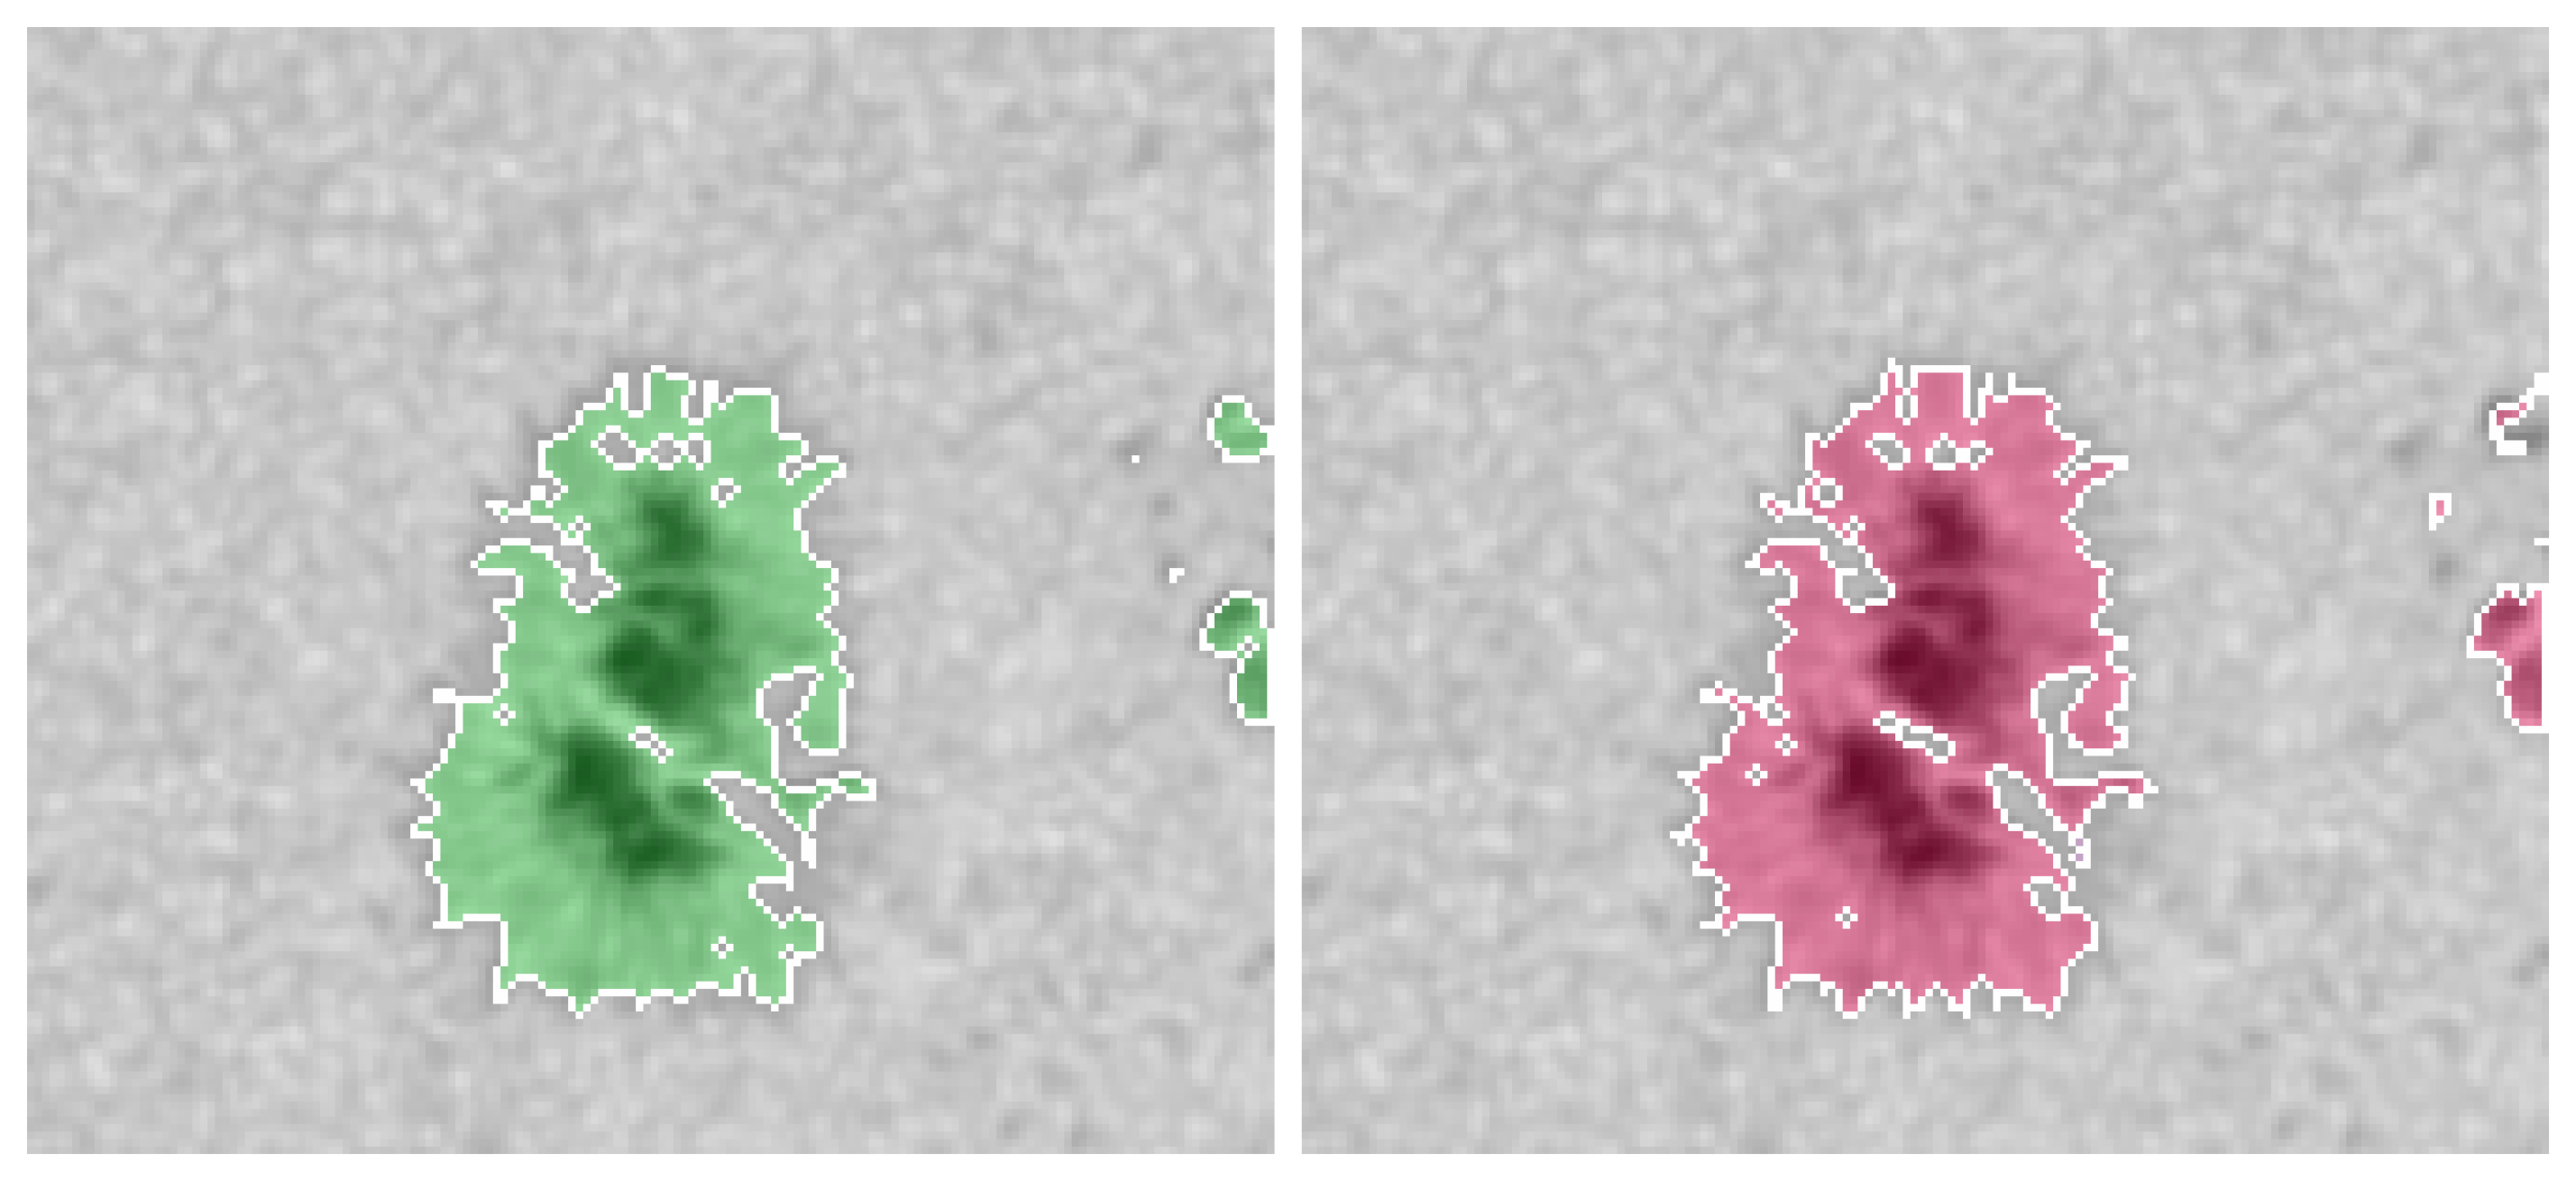
\includegraphics[width=\textwidth]{./pictures/pred-vs-ground}
    \caption{Comparison between the predicted mask (green) and the ground truth (red).}
    \label{fig:pred-vs-ground}
\end{figure}
\begin{figure}[t!]
    \centering
    \captionsetup{justification=centering}
    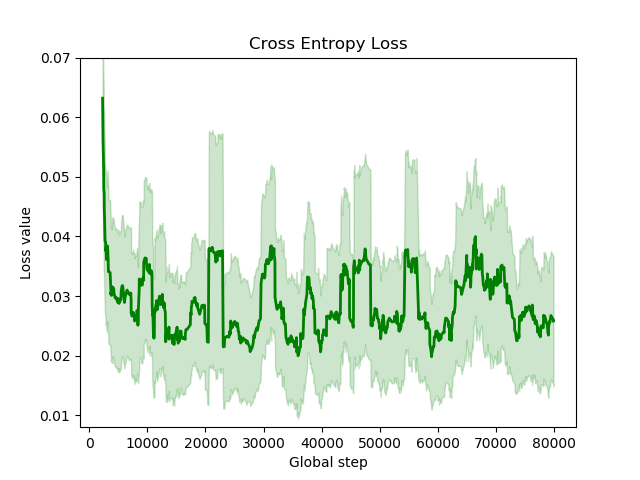
\includegraphics[width=\textwidth]{./pictures/cross-entropy-loss}
    \caption{U-Net convergence curve on the training set.}
    \label{fig:cross-entropy-loss}
\end{figure}
\clearpage
\begin{figure}[h]
    \centering
    \captionsetup{justification=centering}
    \includegraphics[width=\textwidth]{./pictures/workflow}
    \caption{Summary of the training of the segmentation phase}
    \label{fig:workflow}
\end{figure}
\clearpage
\subsection{Sunspot Representations and Classification}
Probably, the part of the sunspot index estimation that requires most expert knowledge is the determination of the number of groups. The setting of the problem is mainly unsupervised, because groups change every day and there is no predefined category that generalizes from one day to another.
\bigbreak
\noindent  Clustering seems a very natural approach for this problem. It is indeed, but it is also desirable to leverage the datasets of annotated sunspot groups that are available online to make the algorithm mimic the way humans cluster sunspots. A sensible form of blending together a supervised model with clustering is by using the labels to create good representations of the data. Specifically, we want to take the image of a sunspot and remap it to a feature vector that optimizes the result of the subsequent step. This can be achieved by training a siamese network that embeds sunspots in a way that separates them according to the configuration of the groups. To guide the neural network in the search of the optimal features to extract, a contrastive loss is applied. After the mapping is performed, clustering can be employed to find the number of groups.
\bigbreak
\noindent At each training episode a ground truth mask that also contains the instances of the clusters is loaded from the dataset. From every group that is present on the disk, an anchor sunspot is randomly chosen. If the sunspot is not alone in the group, a positive example is selected from the same group. Similarly, a negative example is chosen from the other clusters if they exist. A square patch is centered and cropped from the full-disk image for each example that has been sampled. Now, the visual appearence of the sunspot is certainly an important feature, but its position and its total area are crucial as well. So, how can we give this features as inputs to the siamese network? Recent studies have shown that coordinates can be given as input to convolutional neural networks to improve their performance \cite{liu2018intriguing}. Thus, the centroids of each sunspot in heliographic coordinates are appended as a channel to the input tensor (the coordinate value is repeated on the whole channel). The same is done with the value of the area, after having it normalized by the total area of the disk. The final input tensor to the convolutional layers has therefore 4 channels (as it can be seen in Figure~\ref{fig:siamese-workflow}) holding respectively:
\begin{itemize}
  \item 1 channel for the patch of the image that contains the sunspot;
  \item 2 channels for the heliographic latitude and longitude;
  \item 1 channel for the normalized area of the sunspot.
\end{itemize}
After the tensor is propagated, the convolutaional layers produce an intermediate representation that, in turn, passes through two fully connected layers, generating a 5-dimesional embedding as output. This procedure gets repeated for all the selected sunspots and for each one of them the loss tries to pull the positive matches together (low Euclidean distance) while pushing the negative ones apart (high Euclidean distance).
\bigbreak
\noindent At the same time, the convolutional layers are repurposed for classification. The intermediate representation generated by the convolutional layers is also fed to a second, almost identical fully connected block that deals with classification. In this case, the desired output is the modified Z\"{u}rich class (Z component of the McIntosh classification). Identifying the type of sunspot that is being processed is important because the presence of penumbra surrounding the umbra can be derived directly from the class. As always, the classification error (calculated with the standard cross entropy loss) is backpropagated through the layers. Note that the fully connected layers only receive the gradients coming from their own output while the shared convolutional layers accumulate the gradients coming from both the contrastive loss and the cross entropy loss.
\bigbreak
\noindent This type of learning paradigm, where the network solves two or more problems at the same time, is called multitask learning \cite{caruana1997multitask}. It is based on the idea that what is learned for each task can help other tasks be learned better. This is indeed the case for sunspot clustering. In fact, even humans use group classification as an aid in the process of grouping them together.
\bigbreak
\noindent The process of training this ``two-headed'' architecture was very hard, due to the fact that the way positive and negative examples are selected makes a very big impact on the final result. Nonetheless, finally, it was possible to make the network learn both tasks with very good performance. The training curves can be examined in Figure~\ref{fig:siamese-training}.
\begin{figure}[hb!]
  \centering
  \captionsetup{justification=centering}
  \includegraphics[width=\textwidth]{./pictures/siamese-workflow}
  \caption{Summary of the training of the siamese network}
  \label{fig:siamese-workflow}
\end{figure}
\begin{figure}[h!]
    \centering
    \captionsetup{justification=centering}
    \begin{subfigure}[t]{\textwidth}
        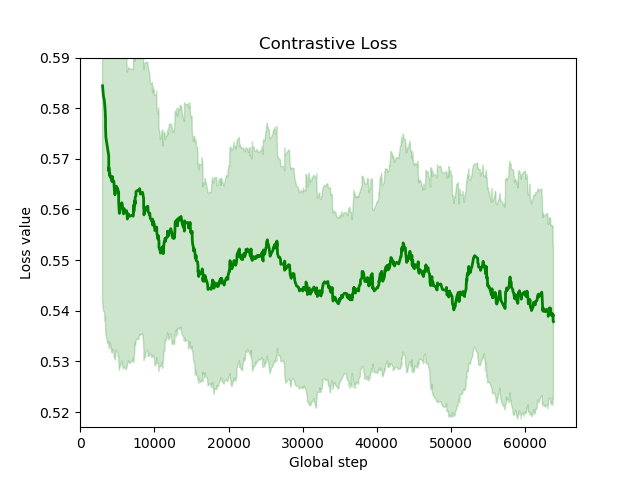
\includegraphics[width=\textwidth]{./pictures/contrastive-loss}
    \end{subfigure}\vspace{3mm}
    \begin{subfigure}[t]{\textwidth}
        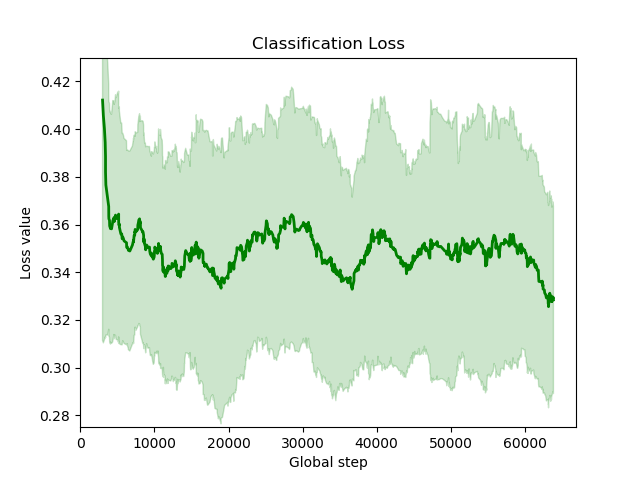
\includegraphics[width=\textwidth]{./pictures/classification-loss}
    \end{subfigure}
    \caption{Multitask siamese network convergence curve. Note that the implementation of the contrastive loss that has been used constrains the minimum possible value to be 0.5}
    \label{fig:siamese-training}
\end{figure}
\clearpage
\section{Automatic Annotation Procedure}
\label{autoannotation}
After both components of the model have been trained, it is time to join them in order to make predictions on unseen data. However, just stacking the U-Net and the siamese network together is not sufficient and other subcomponents are added. In this section we aim at describing in detail all the steps that are necessary to compose a successful annotation algorithm.
\bigbreak
\noindent Contrary to the training phase, the loading routine is now very simple, since it just needs to fetch the image that is annotated and no mask is needed (it is produced automatically). So, the prediction routine starts loading the image and dividing it into patches, while the parameters of the two neural networks get restored from selected checkpoints. One by one, the patches get sent into the U-Net that takes care of the first segmentation stage. As soon as the whole image has been evaluated, the mask gets reconstructed from the patches. Note that, since the U-Net outputs probabilities, every pixel has a continuous value (between 0 and 1) that needs to be rounded with a threshold in order to obtain a mask where the background has value 0 and the sunspot areas have value 1.
\bigbreak
\noindent At this point, we know with good confindence that the parts of the image that have been highlighted from the U-Net contain one or more sunspots each. To use this information for the subsequent steps we first need to convert it to a more usable form. The mask is, scanned looking for connected componets of pixels with value 1. At the same time, statistics are extracted for every component and the data is organized in an array. It is precisely from this information that the inputs for the siamese network are created. In fact, similarly to what was done during training time, the input channels are built using respectively a centered patch, the coordinates of the centroid and the area of the connected components. Coordinates are now in pixel space so they need to be translated to the heliographic system via trigonometry. When this is done, the data is forwarded through the convolutional layers of the siamese network and then the two fully connected heads are evaluated in parallel. The network outputs both the embeddings and the classes of each connected component.
\bigbreak
\noindent From this moment on, the computaton splits in two branches, one that seeks to refine the quality of the segmentation to yield the number of single sunspots, the other that finds the number of groups and assigns each sunspot to one of them.
\begin{figure}[ht!]
  \centering
  \captionsetup{justification=centering}
  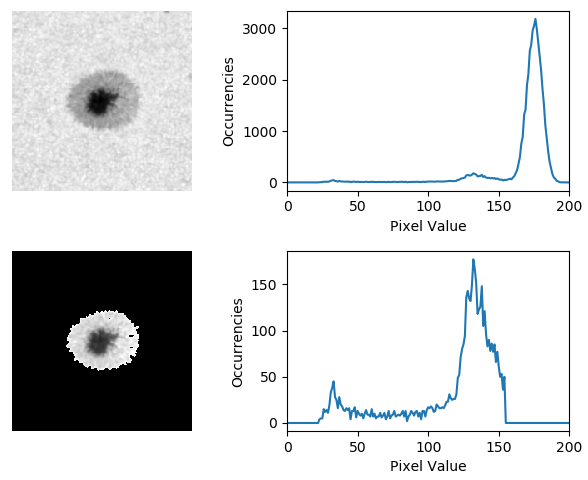
\includegraphics[width=\textwidth]{./pictures/histograms}
  \caption{Comparison between histograms of the same patch, with or without the mask}
  \label{fig:histograms}
\end{figure}
Refining the quality of the segmentation mask means, in this context, to be able to separate the umbra from the penumbra of each connected component of pixels generated by the U-Net. This operation is important because more than one umbrae can be surrounded by the same penumbrae, affecting the sunspot count. First, it is necessary to understand if the sunspot exhibits or not the penumbra. This is easy considered that we can leverage the classification produced by the siamese network together with some simple heuristic concerning the area of the sunspot.
\bigbreak
\noindent Classes \textbf{A} and \textbf{B} imply that the sunspots of the group do not have penumbra while classes \textbf{C} to \textbf{H} all expect penumbra. Small sunspots that usually locate at the periphery of groups are directly discarded with some threshold on the value of the area since we assume that they are very unlikely to carry more than one umbra. This knowledge enables us to segment the connected component using its histogram. In fact, since the division between umbra and penumbra creates a strong intensity discontinuity, the cut-off value is evident in the histogram if the mask of the whole sunspot is known a priori. Referring to Figure~\ref{fig:histograms} as an aid to visualization, the two peaks that can be seen around pixel value 30 and 130 are respectively the umbra and the penumbra. Given this knowledge of the problem we can proceed with two approaches, either fitting two gaussians and assigning each pixel to the most likely one, or simply perforoming clustering in one dimension fixing the number of clusters to the value 2. Both solutions were explored during the development of this work but in the end clustering was selected because, despite being simpler, it yields the same performance.
\bigbreak
\noindent At the end, the refinement of the segmentation step reduces to running k-means on the mask generated by the U-Net. The two clusters of pixels are then used to create a new mask that only highlights umbras, and the number of connected components is recalculated from it.
\bigbreak
\noindent The second branch of the procedure finds the number of groups and assigns each sunspot (connected component of pixels) to one of them, using the embeddings created by the siamese network. Those embeddings are created to optimize the positions of the connected components in a 5-dimensional Euclidean space. As already treated in the previous section, the optimization operated by the siamese network lies in the fact that sunspots belonging to the same group should be close together in the Euclidean space. This is, once again, a great opportunity to unleash the potential of clustering algorithms. However, the main difficulty here is that the number of clusters is not known beforehand, because it is indeed the value that we want to calculate.
\bigbreak
\noindent DBSCAN seems like a very good match for this problem. In fact, it just needs two parameters: $eps$ ($\varepsilon$) which can be estimated statistically on the validation set (see next section) and $minPts$ which is trivially set to 0 (otherwise groups composed by a lone sunspot would be interpreted as outliers). Given the parameters and the embeddings as inputs, DBSCAN reliably returns the number of clusters that is useful for later computations.
\bigbreak
\noindent Now that the image has been annotated and the number of groups and single sunspots is known it is sufficient to find the personal reduction coefficient to be able to calculate the final value of the relative sunspot number. The estimation of the personal reduction coefficient and the $eps$ ($\varepsilon$) parameter for DBSCAN are addressed in the next section.

\section{Parameter Estimation}
The validation set provides an exceptional opportunity for the estimation of parameters. In fact, many instances of the algorithm can be run using the data that was held out from the training set, so the variation in performance can be assessed. Various combinations of parameters can be evaluated and the best model can be then used to draw the final results on the test set.
Among the others, two parameters have been studied in detail in this work:
\begin{itemize}
  \item the $eps$ ($\varepsilon$) parameter for DBSCAN that represent the minimum distance between two points for them to be considered neighbors;
  \item the personal reduction coefficient ($K$) of the algorithm, compared to the international sunspot number provided by SILSO.
\end{itemize}
These two parameters are not independent from each other and therefore they were tested in two consecutive phases, both on the whole validation set.
\bigbreak
\noindent The first one that needed to be assessed was the value of $eps$. The number of clusters detected from DBSCAN dramatically depends on this parameter, so optimizing it is vital to improve the final performance. Although the variable that drives the performance is the number of clusters, we didn't use it as the measure to optimize $eps$ because it is not informative enough. Instead, the Adjusted Random Index (ARI), a performance index that takes into account the configuration of points inside the clusters and compares it to the ground truth was used. ARI is defined as:
\begin{equation}
ARI = \frac{RI-\mathbb{E}[RI]}{max(RI)-\mathbb{E}[RI]}
\end{equation}
where $RI$ (Rand Index) is the number of pairs of objects that are either in the same group or in different groups in both partitions divided by the total number of pairs of objects. The ARI performs a correction with respect to the Rand index in order to account for the variability of the expected value of two random partitions. Thus, the ARI has a value close to 0 for random labeling independently of the number of clusters and exactly 1 when the clusterings are identical.
\bigbreak
\noindent We tested the algorithm 50 times on the whole validation set, each time with a different value for the $eps$ parameter. The results are shown in Figure~\ref{fig:eps-ari}. After the estimation of the curve it is possible to take the value that maximizes the performance index and use it as input for the subsequent tests.
\bigbreak
\noindent After $eps$, we proceded to estimate the value of the reduction coefficient $K$ using a similar procedure. This time, instead of maximizing some performance index, the task is to minimize the deviation of our calculation of the sunspot number from the international sunspot index provided by SILSO. This can be achieved using the root-mean-square (RMS) error between the two calculations over the whole validation set. The procedure was repeated 100 times with values of $K$ ranging from 0 to 2 (Figure~\ref{fig:k-rms}). The optimal minimal error is attained when the $K$ coefficient takes the value 0.58. Such a low value for $K$ is explained by the fact that the images that have been used by our algorithm come from the best observatories in the world. Depending on the optics of the telescope, the amount of detail that can be resolved changes. So, in general, the better the optics, the more sunspots it captures. For this reason, the estimation our algorithm provides is high, and therefore it should be multiplied by a low value to align to the international sunspot number.\clearpage
\begin{figure}[ht!]
  \centering
  \captionsetup{justification=centering}
  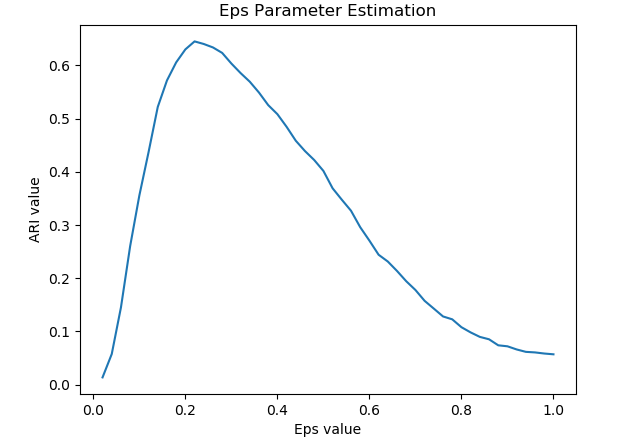
\includegraphics[width=\textwidth]{./pictures/eps-ari-copy}
  \caption{ARI value for varying $eps$ values}
  \label{fig:eps-ari}
\end{figure}
\begin{figure}[h!]
  \centering
  \captionsetup{justification=centering}
  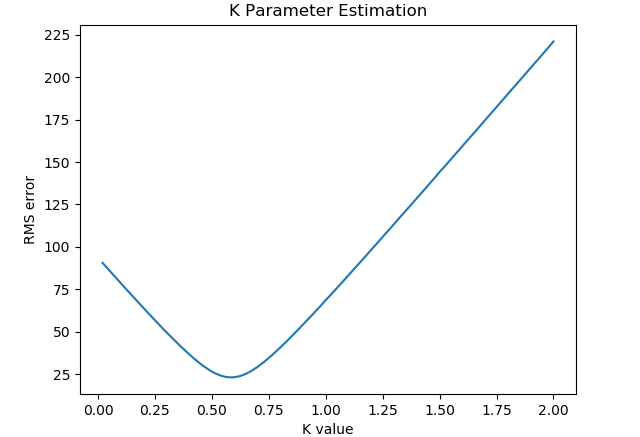
\includegraphics[width=\textwidth]{./pictures/k-rms-copy}
  \caption{RMS error value for varying $K$ value}
  \label{fig:k-rms}
\end{figure}

% \chapter{Results and Future Work}
\label{capitolo8}
\thispagestyle{empty}
\section{Results}

\section{Future Work}

% \chapter{Future Work}
\label{capitolo9}
\thispagestyle{empty}
- look at other clustering methods that solve the density problem
- use more data, incorporate past cycles
- use triplet loss instead of contrastive or hybrid siamese network
- use heterogeneous annotations
- try to train instance segmentation inside the network
- use NOAA sunspot dataset too
- use STARA and try to replicate the same experiments
- a more accurate study on the minimization of the dependencies inside the dataset
- end to end training
- integrate penumbra
- look into why eps does not gingilla 

\cleardoublepage
% ---- Bibliography ----
\pagestyle{plain}
\addcontentsline{toc}{chapter}{Bibliography}
\bibliographystyle{unsrt}
\bibliography{bibliography}

%\nocite{*}

\appendix

\pagestyle{fancy}
\fancyfoot{}
\renewcommand{\chaptermark}[1]{\markboth{\appendixname\ \thechapter.\ #1}{}}
\renewcommand{\sectionmark}[1]{\markright{\thesection.\ #1}}
% \fancyhead[LE,RO]{\bfseries\thepage}

\fancyhead[RE]{\bfseries\leftmark}
\fancyhead[LO]{\bfseries\rightmark}
\renewcommand{\headrulewidth}{0.3pt}

\chapter{Glossary}
\label{appendiceA}
\thispagestyle{empty}

The definitions in this glossary are taken from NOAA's space weather glossary \cite{NOAAglossary}.\\


\newenvironment{myindentpar}[1]%
{\begin{list}{}%
        {\setlength{\leftmargin}{#1}}%
        \item[]%
}
{\end{list}}


\textbf{Active Region:}
\begin{myindentpar}{1cm}
  A localized, transient volume of the solar atmosphere in which plages, sunspots, faculae, flares, etc. may be observed.
\end{myindentpar}

\textbf{Aurora:}
\begin{myindentpar}{1cm}
A faint visual (optical) phenomenon on the Earth associated with geomagnetic activity, which occurs mainly in the high-latitude night sky. Typical auroras are 100 to 250 km above the ground. The Aurora Borealis occurs in the northern hemisphere and the Aurora Australis occurs in the southern hemisphere.
\end{myindentpar}

\textbf{Corona:}
\begin{myindentpar}{1cm}
  The outermost layer of the solar atmosphere, characterized by low densities and extraordinarily high temperatures that extends to several solar radii. The heating of the corona is still a mystery. The shape of the corona is different at solar maximum and at solar minimum.
\end{myindentpar}

\textbf{Coronal Hole:}
\begin{myindentpar}{1cm}
  An extended region of the corona, exceptionally low in density (large open "gaps"), and associated with photospheric regions. Coronal holes are closely associated with those regions on the Sun that have an "open" magnetic geometry, that is, the magnetic field lines associated with them extend far outward into interplanetary space, rather than looping back to the photosphere. Ionized material can flow easily along such a path, and this in turn aids the mechanism that causes high speed solar wind streams to develop.
\end{myindentpar}

\textbf{Coronal Mass Ejection:}
\begin{myindentpar}{1cm}
  An observable change in coronal structure that occurs on a time scale between a few minutes and several hours, and involves the appearance of a new discrete, bright, white light feature in the coronagraph field of view, that displays a predominantly outward motion. The solar corona material is massive in size (they can occupy up to a quarter of the solar limb), and frequently accompanied by the remnants of an eruptive prominence, and less often by a strong solar flare. The leading edges of fast-moving CMEs drive giant shock waves before them through the solar wind at speeds up to 1200 km per second. Some astronomers believe that CMEs are the crucial link between a solar disturbance its propagation through the heliosphere, and the effects on the Earth.
\end{myindentpar}

\textbf{Differential Rotation:}
\begin{myindentpar}{1cm}
  The change in solar rotation rate with latitude. Low latitudes rotate at a faster angular rate (approx. 14 degrees per day) than do high latitudes (approx. 12 degrees per day). For example, the equatorial rotation period is 27.7 days compared to 28.6 days at latitude 40 degrees.
\end{myindentpar}

\textbf{Disk:}
\begin{myindentpar}{1cm}
  The visible surface of the Sun (or any heavenly body) projected against the sky.
\end{myindentpar}

\textbf{Eruptive:}
\begin{myindentpar}{1cm}
  Solar activity levels with at least one radio event and several chromospheric events per day.
\end{myindentpar}

\textbf{Facula:}
\begin{myindentpar}{1cm}
  A bright cloud-like feature located a few hundred km above the photosphere near sunspot groups, seen in white light. Facula are seldom visible except near the solar limb, although they occur all across the Sun. Facula are clouds of emission that occur where a strong magnetic field creates extra heat (about 300 degrees K above surrounding areas).
\end{myindentpar}

\textbf{Filament:}
\begin{myindentpar}{1cm}
  A mass of gas suspended over the photosphere by magnetic fields and seen as dark lines threaded over the solar disk. A filament on the limb of the Sun seen in emission against the dark sky is called a prominence.
\end{myindentpar}

\textbf{Flux:}
\begin{myindentpar}{1cm}
  The rate of flow of a physical quantity through a reference surface.
\end{myindentpar}

\textbf{Geomagnetic Field:}
\begin{myindentpar}{1cm}
  The magnetic field observed in and around the Earth. The intensity of the magnetic field at the Earth's surface is approximately 0.32 gauss at the equator and 0.62 gauss at the north pole.
\end{myindentpar}

\textbf{H-alpha:}
\begin{myindentpar}{1cm}
  This absorption line of neutral hydrogen falls in the red part of the visible spectrum and is convenient for solar observations. The H-alpha line is universally used for observations of solar flares and prominences.
\end{myindentpar}

\textbf{Helioseismology:}
\begin{myindentpar}{1cm}
  A method for studing the Sun by utilizing waves that propagate throughout the star to measure its invisible internal structure and dynamics.
\end{myindentpar}

\textbf{Limb:}
\begin{myindentpar}{1cm}
  The edge of the solar disk.
\end{myindentpar}

\textbf{Magnetogram:}
\begin{myindentpar}{1cm}
  Solar magnetograms are a graphic representation of solar magnetic field strengths and polarity.
\end{myindentpar}

\textbf{Penumbra:}
\begin{myindentpar}{1cm}
  The sunspot area that may surround the darker umbra or umbrae. It consists of linear bright and dark elements radial from the sunspot umbra.
\end{myindentpar}

\textbf{Plage:}
\begin{myindentpar}{1cm}
 An extended emission feature of an active region that exists from the emergence of the first magnetic flux until the widely scattered remnant magnetic fields merge with the background. This bright feature is found in the vicinity of virtually all active sunspot groups and occurs on a larger scale and are brighter than facula. Plage is French for "beach," because each plage looks like light-colored sand against the darker structures around them.
\end{myindentpar}

\textbf{Plasma:}
\begin{myindentpar}{1cm}
  Any ionized gas, that is, any gas containing ions and electrons.
\end{myindentpar}

\textbf{Prominence:}
\begin{myindentpar}{1cm}
  A term identifying cloud-like features in the solar atmosphere. The features appear as bright structures in the corona above the solar limb and as dark filaments when seen projected against the solar disk.
\end{myindentpar}

\textbf{Quiet:}
\begin{myindentpar}{1cm}
  Solar activity levels with less than one chromospheric event per day.
\end{myindentpar}

\textbf{Solar Cycle:}
\begin{myindentpar}{1cm}
  The approximately 11-year quasi-periodic variation in frequency or number of solar active events.
\end{myindentpar}

\textbf{Solar Maximum:}
\begin{myindentpar}{1cm}
  The month(s) during the solar cycle when the 12-month mean of monthly average sunspot numbers reaches a maximum.
\end{myindentpar}

\textbf{Solar Minimum:}
\begin{myindentpar}{1cm}
  The month(s) during the solar cycle when the 12-month mean of monthly average sunspot numbers reaches a minimum.
\end{myindentpar}

\textbf{Umbra:}
\begin{myindentpar}{1cm}
  The dark core or cores (umbrae) in a sunspot with penumbra, or a sunspot lacking penumbra.
\end{myindentpar}

\textbf{White-Light:}
\begin{myindentpar}{1cm}
  Sunlight integrated over the visible portion of the spectrum (4000 - 7000 angstroms) so that all colors are blended to appear white to the eye.
\end{myindentpar}

\chapter{Documentazione della programmazione}
\label{appendiceB}
\thispagestyle{empty}

\chapter{Helios Processing Pipeline}
\label{appendiceC}
\thispagestyle{empty}
This appendix describes the first part of the work that was done at the Helios observatory of the European Space Agency. The observatory belongs to the CESAR (Cooperation through Education in Science and Astronomy Research) initiative, whose objective is to provide students from european secondary schools and universities with hands-on experience in Astronomy research in general and in Radio Astronomy and Optical Astronomy in particular. Helios was installed at ESAC (European Space Astronomy Centre) in 2012 and includes two telescopes (Figure wanama):
\begin{itemize}
  \item Coronado Solarmax II 90, H-alpha, double stack, with specifications:
  \begin{itemize}
    \item Aperture: 90mm
    \item Focal Length: 800mm
    \item Bandwidth: \textless0.5 \AA
  \end{itemize}
  \item Bresser AR-102, visible (white-light), with specifications:
  \begin{itemize}
    \item Aperture: 102mm
    \item Focal Length: 1000mm
    \item Solar Filter: BAADER AstroSolar Safety Filter
  \end{itemize}
\end{itemize}
\bigbreak
The two telescopes are mounted on the same robotic arm (Figure wanama) and are very different from each other. The main difference is in the type of filter they have on board. On the one hand, the filter that comes with the Coronado Solarmax isolates the H-alpha band, a deep-red visible spectral line. H-alpha is particularly useful in solar astronomy because it enables the observation of the atmosphere of the Sun. On the other hand, the filters that are used for white-light observation do not reduce the portion of the specturm that enters the scope, but rather decrease the intesity of the radiation. Therefore each pixel of the sensor, attached at the bottom of the scope, receives the whole visible spectrum and integrates it to obtain the total intensity.
\bigbreak
\begin{figure}[t!]
    \centering
    \captionsetup{justification=centering}
    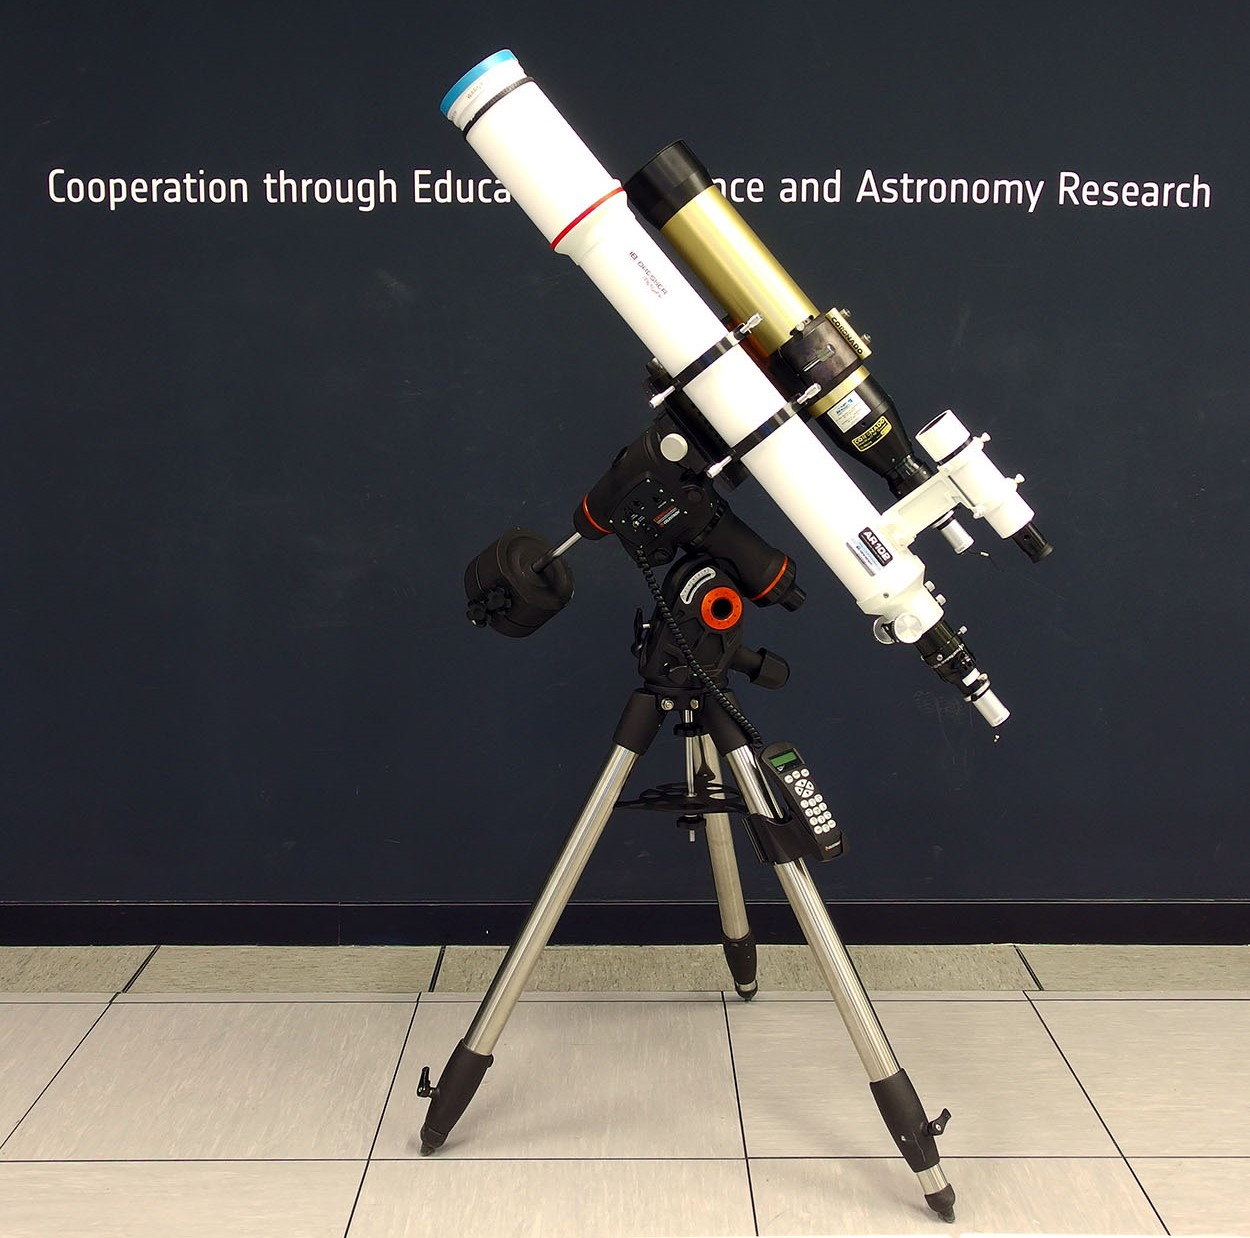
\includegraphics[height=0.4\textheight]{./pictures/solar-telescopes}
    \caption{A picture of the two telescopes}
    \label{fig:pred-vs-ground}
\end{figure}
Given these differences, dedicated processing techniques are used for each telescope. Nonetheless, the preliminary steps of the two pipelines are shared, although with different parameters, and they are therefore presented together. In fact, we can logically divide the pipelines in two phases (which are treated in the next sections):
\begin{itemize}
  \item \textbf{Preliminary adjustments}, performed for both telescopes with different parameters;
  \item \textbf{Feature enhancement}, dedicated for each telescope.
\end{itemize}

\section{Preliminary Adjustments}
The first phase of the processing starts with a set of quality control checks. For each image we need to make sure that they are not corrupted or completely black, since files could be damaged during the transfer from the observatory to the servers that are allocated for the processing. Then, a second check, called cloud control, is performed to retain only the images where the Sun is perfectly visible, and discard the cloudy ones.
\bigbreak
Once it is certain that the images are up to standard, the pipeline proceeds to perform some corrections that are necessary to remove the artifacts introduced by the sensor. In fact, even the best sensors suffer from variations in the pixel sensitivity of the detector and distortions in the optical path. Luckily, is possible to account for these errors unsing two techniques that are really popular in digital photograpy: \textbf{dark-frame subtraction} and \textbf{flat-field correction}. The former tries to minimize the noise due to defective pixels and dark currents, while the latter adjusts for the relative sensitivity of pixels. The dark-frame is created by taking long exposure images in con complete darkness, or, in this case, when the lid of the telescope is on. The flat-field, instead, is generated attaching an omogeneous light source over the instrument, to measure how much each pixel reacts to it. Thus, two calibration images are used to adjust the images with the following formula:
\begin{equation}
C = \frac{(R - D)}{(F - D)}
\end{equation}
where $C$ is the corrected image, $R$ is the raw image, and $F$ and $D$ are the flat-field and the dark-frame respectively.
\bigbreak
The third subphase of the preliminary adjustments phase deals with image centering and axial tilt correction. Although, as explained in Appendix D, the telescope itself and the master control program already account for the tracking of the Sun, the limited accuracy of mechanical arms makes it necessary to use image processing techniques to align and center the solar disk to the frame. Moreover, in this case, centering the image is made easier by the fact that the shape of the object we are looking for is known and its size can be calculated with simple geometry. In fact, first, the sun can be considered a sphere, since its oblateness is neglectable; and second, the size of the appearent radius can be determined from the Sun-Earth distance. For the latter calculation it is sufficent to know the radius at one point of the orbit (we used the perihelion), and remember that the appearent size of an object is proportional to its distance. Therefore the radius can be calculated as:
\begin{equation}
  R = R_p\frac{d}{d_p}
\end{equation}
where $R$ is the desired radius in pixels at distance $d$, and $R_p$ and $d_p$ are respectively the radius and the distance at perihelion.
\bigbreak
Knowing the appearent radius for each day, it is possible to build a dynamic template of the disk, and template matching can be applied to find the center of the Sun in pixel coordinates. Also, the radius can be used to determine the size of the patch to be cropped in order to obtain an image in which the Sun is centered. The perfect alignment is achieved by rotating the resulting image by an angle that is equal to the axial tilt.

\section{Feature Enhancement}
\subsection{White-light}















- mean and std dev
- gradient sharpening
- limb darkening correction




\subsection{H-alpha}

- off limb emission enhancement
- kernel sharpening

% Given these differences, dedicated processing techniques are used to extract specific features from the raw images of each telescope.  In fact, the two pipelines
























% end

% \chapter{Master Control Program}
\label{appendiceD}
\thispagestyle{empty}
\noindent Apart from the two telescpes described in Appendix C, the Helios solar observatory is composed by a dome, a mount, a weather station and two camera sensors (one for each telescope). Here are the specifications:
\begin{itemize}
  \item a Scopedome 3M dome;
  \item a Celestron CGEM mount;
  \item a AAG CloudWatcher weather station.
  \item two 2 QHY5-II-M planetary cameras with a 1/2 CMOS sensor;
\end{itemize}
All these components come with dedicated proprietary software programs to control them. The problem with these programs is that, apart from some predefined functionality, they are not able to work together. Therefore, in order to fully automate the observatoy, it was necessary to build a dedicated control program.
\bigbreak
\noindent All the hardware was selected according to its capability of being programmed. The protocol that was used in order for the master control program to interface with the hardware is called ASCOM (Astronomy Common Object Model). ASCOM establishes a set of vendor, language and platform independen interface standards for drivers that provide plug-and-play control of astronomical instruments and related devices.
\bigbreak
\noindent The master control program is a very large project, that I started during 2018 and is still ongoing. During my internship I was able to program the connection to the components and a part of the user interface that lets the operator control the observatory manually. For what concerns the automation of the daily observation process, I focused on the improvement of the tracking of Sun.
\bigbreak
\noindent Some tracking capabilities were already offered by the Celestron mount. In fact, once the telescope has slewed to some coordinates, it is able to follow that particular point in the sky, regardless of the rotation of the Earth. This functionality is called tracking, and it is included in any modern mount. The telescope moves thanks to a set of motors and gears that are embedded inside the robotic arm. Like any mechanism, it has imperfections and tolerances, that make the accuracy of the tracking is bounded.
\bigbreak
\begin{figure}[t!]
    \centering
    \captionsetup{justification=centering}
    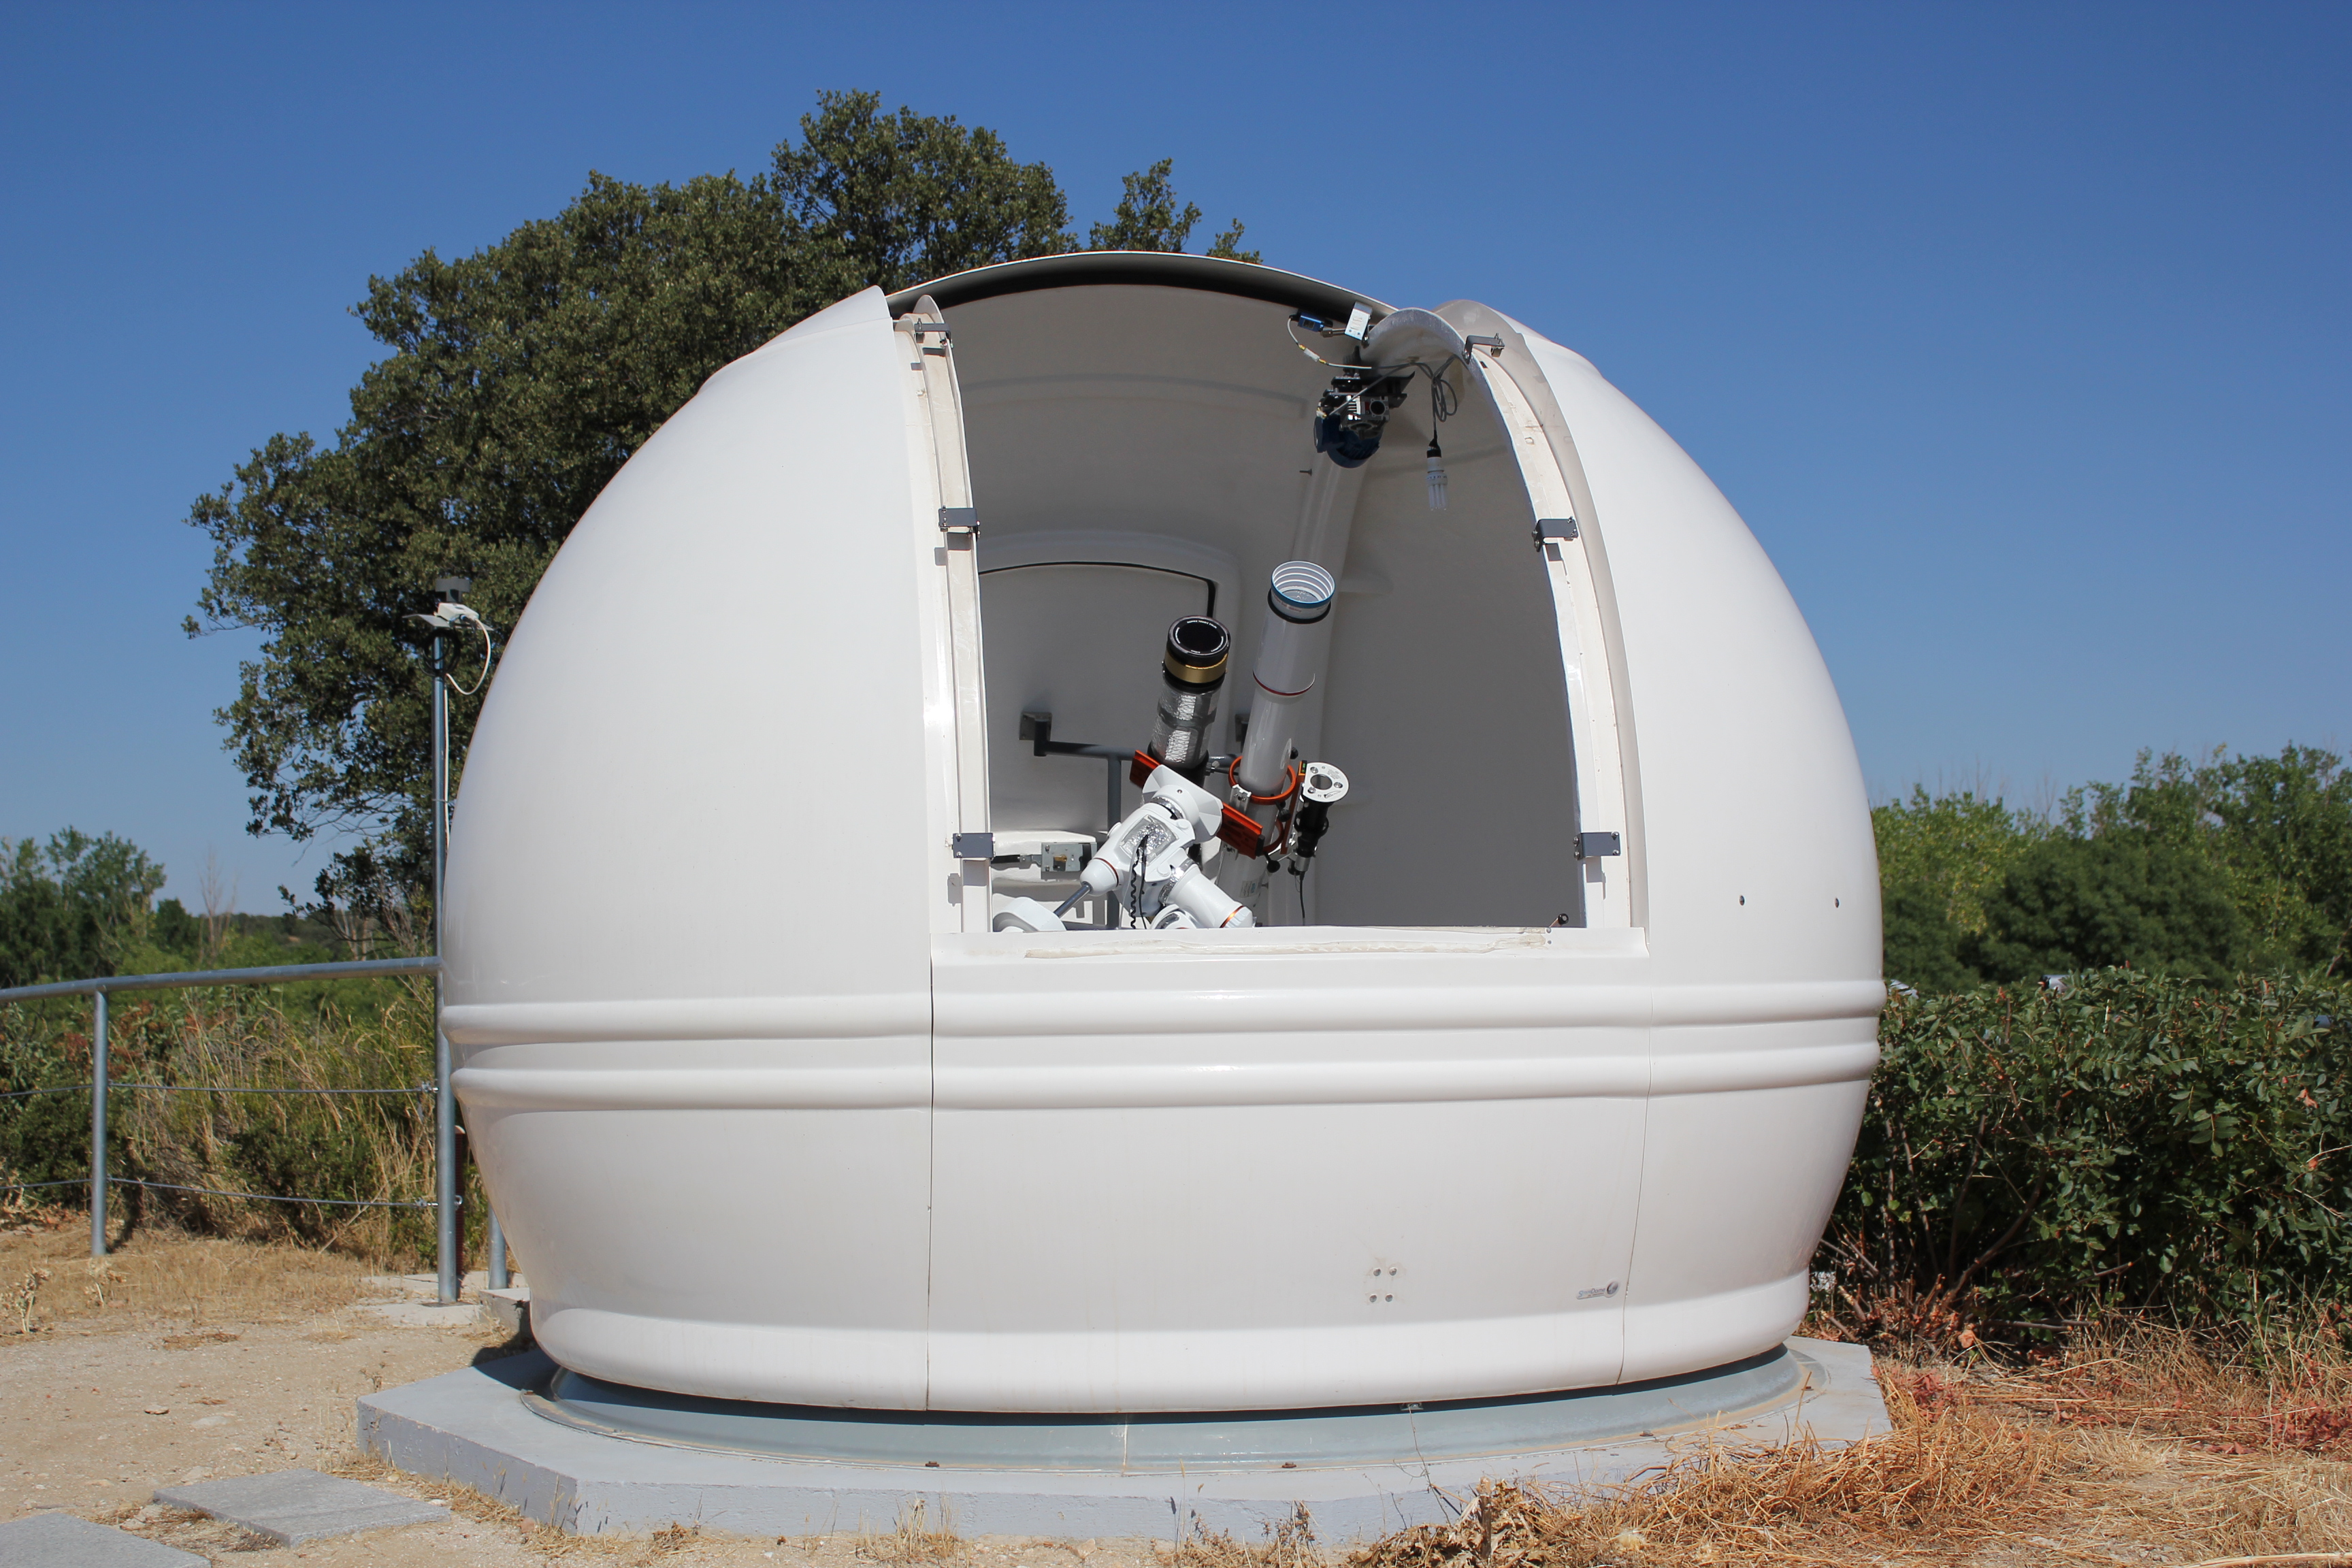
\includegraphics[width=\textwidth]{./pictures/helios}
    \caption{An image of the Helios observatory performing daily observation}
    \label{fig:halpha-visible}
\end{figure}
\noindent The limitations of the mechanical tracking resulted in misalignments in the images, and in some cases in the Sun ending out of the field of view. To address this problem software can come to the aid of hardware. In fact, the two camera sensors stream images in real time from the scope to the control program. As shown in Appendix C, it is fairly easy to find the coordinates of the center of the disk. Hence, it is also possible to calculate the correction that should be applied by the mount to place it back to the center of the frame. In fact, using the same reasoning as in \eqref{eq:radpix}, we can compute how many radians correspond to each pixel of the image and, after some coordinate translation, instruct the telescope to slew back to the Sun.
\bigbreak
\noindent The development of the master control program for is being continued by the interns that followed me at the Helios observatory.

% \chapter{Esempio di impiego}
\label{appendiceE}
\thispagestyle{empty}

% \chapter{Datasheet}
\label{appendiceF}
\thispagestyle{empty}


\end{document}
